\documentclass{article}
	\title{CamelStudioX Tutorial}

\usepackage{graphicx}
\usepackage{subfigure}
\usepackage{float}
\usepackage{geometry}
\geometry{a4paper,left=2cm,right=2cm,top=2cm,bottom=2cm}

\begin{document}
	
	\maketitle
	\section{System Requirements}
		macOS version should be $\geq10.12.2$.
	\section{Installation}
		We strongly advise you to make sure that \textbf{CamelStudioX} is installed in the \textbf{Application} directory, which \textbf{CamelStudioX} can perform reliably.

		\begin{figure}[h]
			
			\begin{minipage}[h]{0.5\linewidth}
				\centering
				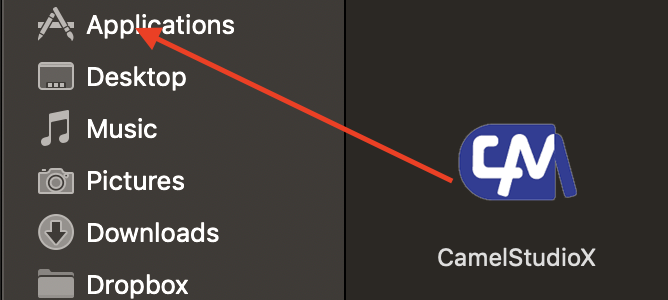
\includegraphics[width=.75\textwidth]{Installation.png}
				\caption{Install CamelStudioX to Application}
			\end{minipage} 
			\begin{minipage}[h]{0.5\linewidth}
				\centering
				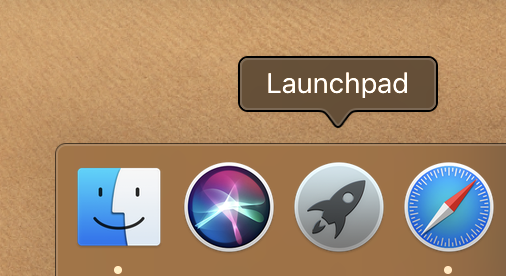
\includegraphics[width=.62\textwidth]{LaunchPad}
				\caption{LaunchPad}
			\end{minipage}
		\end{figure}
			
		What's more, with \textbf{CamelStudioX} installed in \textbf{Application}, you can just click \textbf{LaunchPad} on your dock and then click \textbf{CamelStudioX} to launch it.
		
		\begin{figure}[h]
			\centering
			
		\end{figure}
		
		\begin{figure}[h]
			\centering
			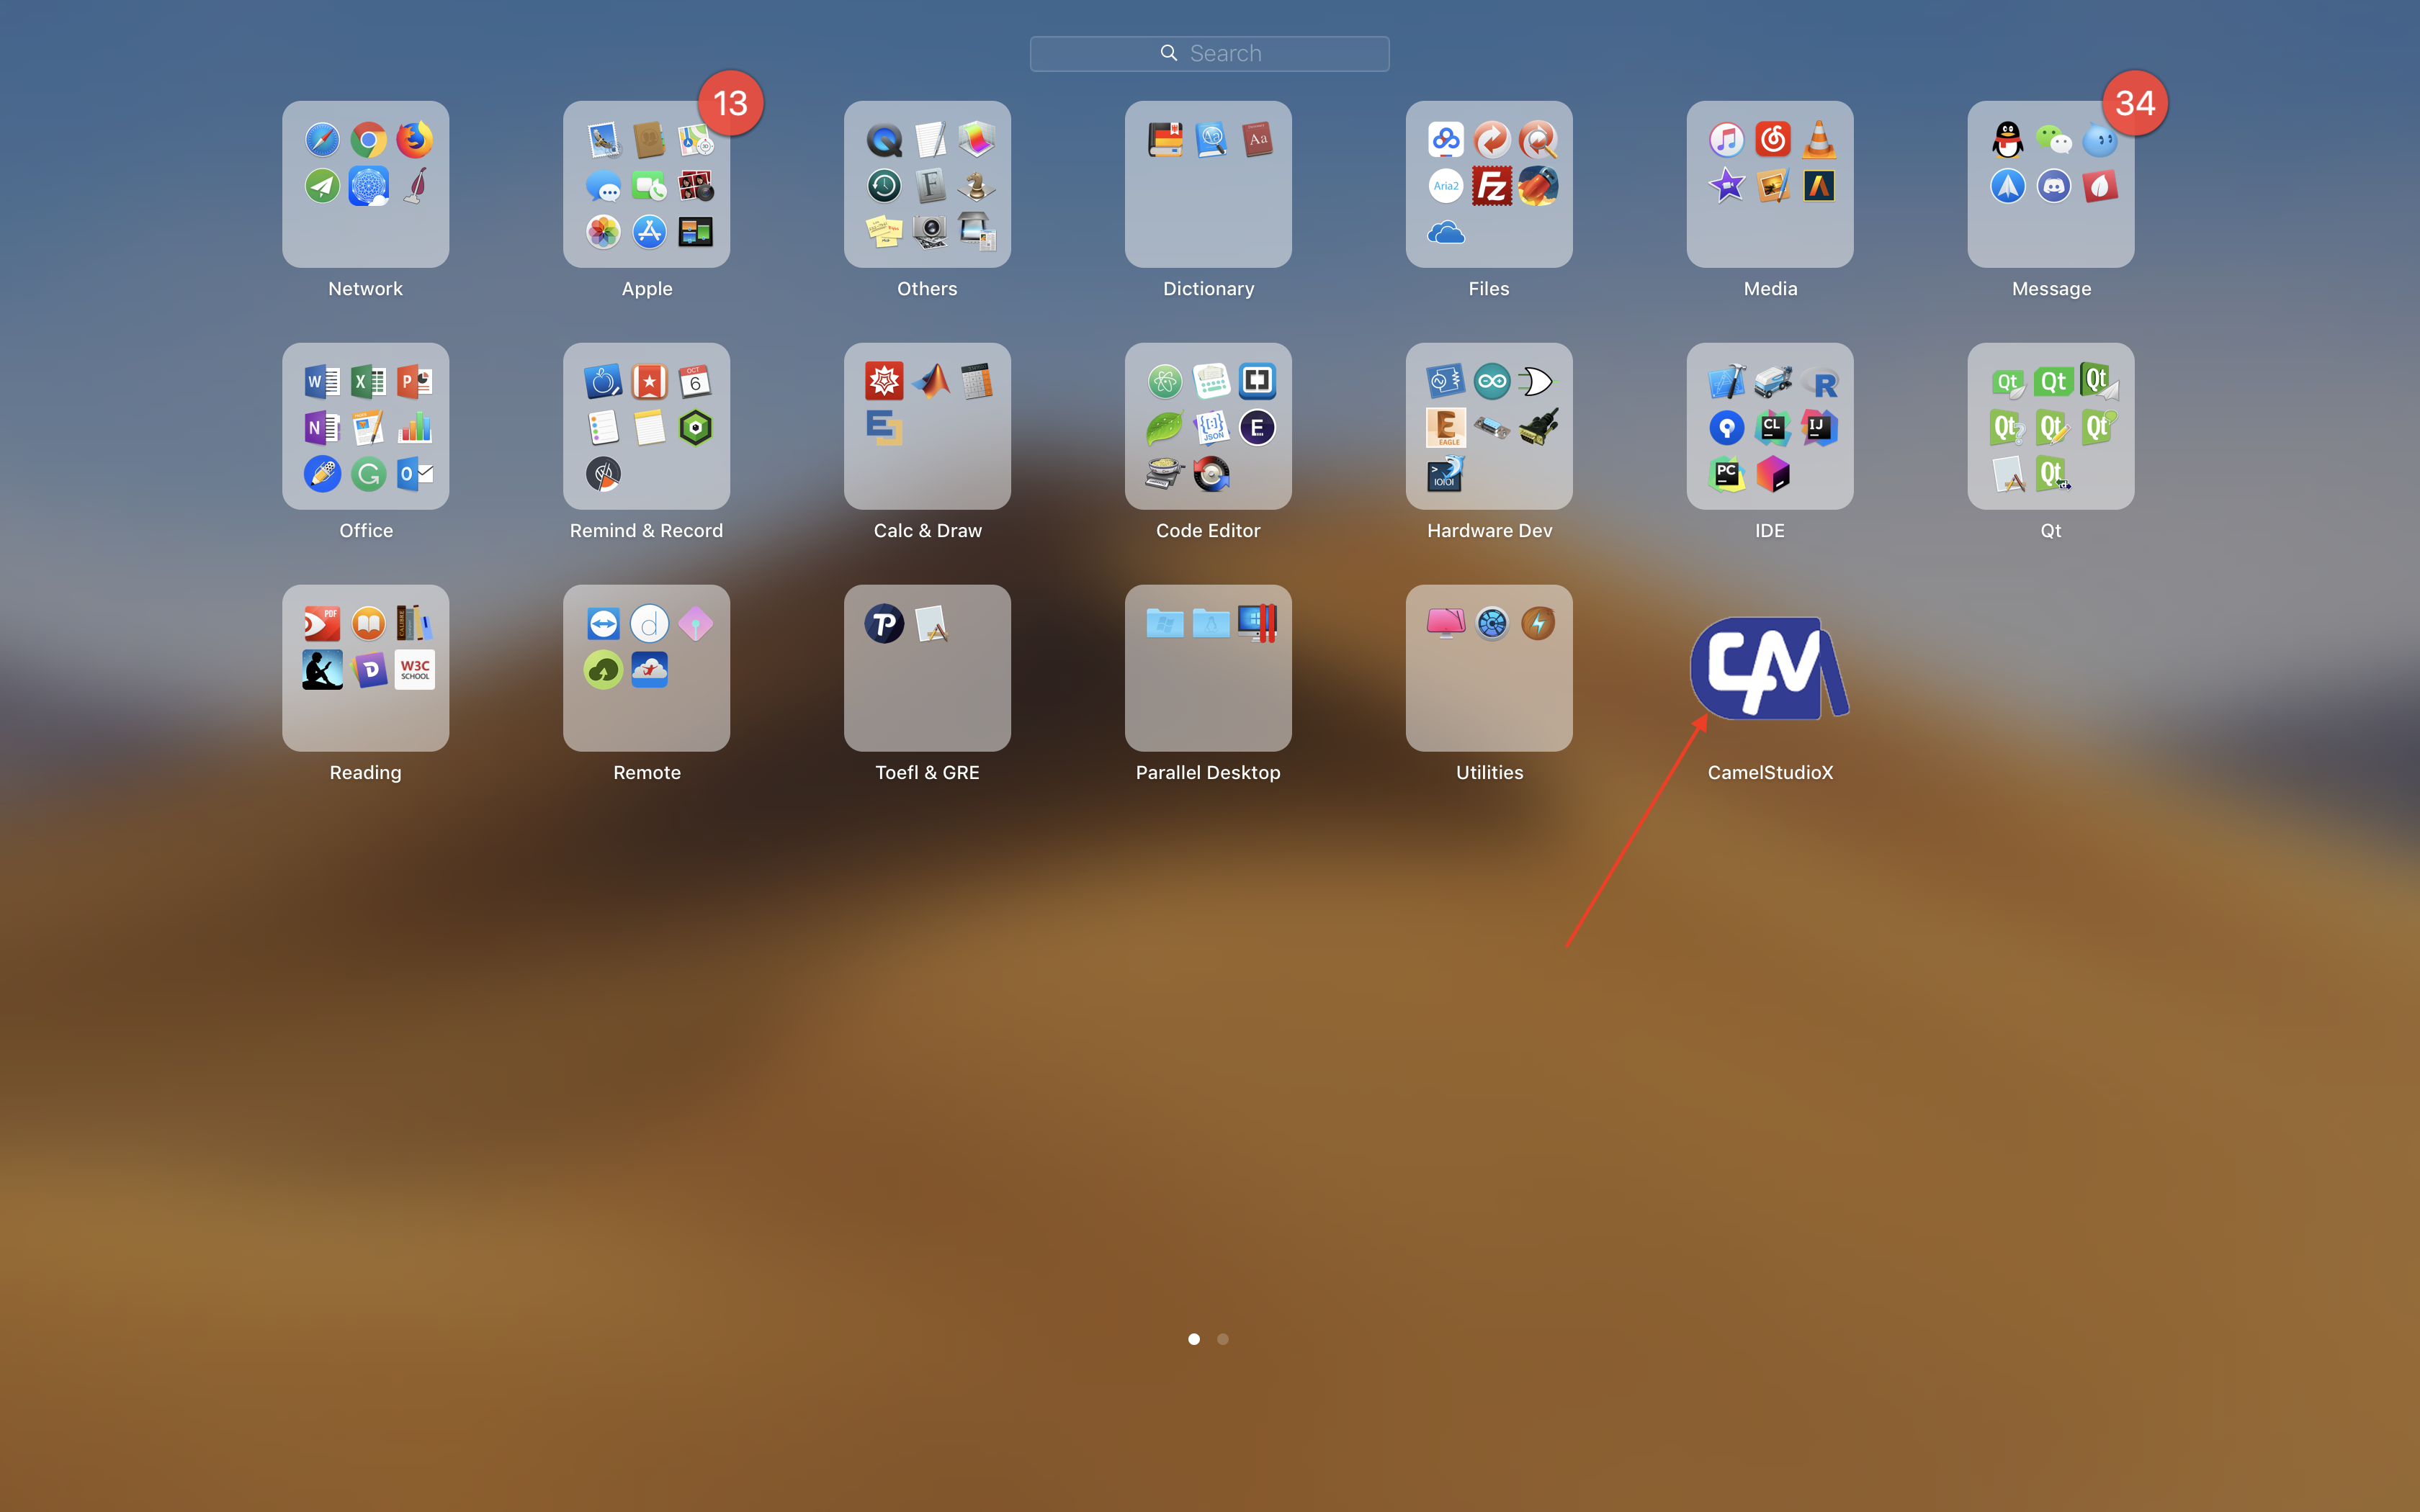
\includegraphics[width=.8\textwidth]{InLaunchPad.png}
			\caption{CamelStudioX in LaunchPad}
		\end{figure}
	
	\newpage
	\section{Welcome Window}
	
	\textbf{CamelStudioX} shows you a welcome window when it is launched.
		
	\begin{figure}[!h]
		\centering
		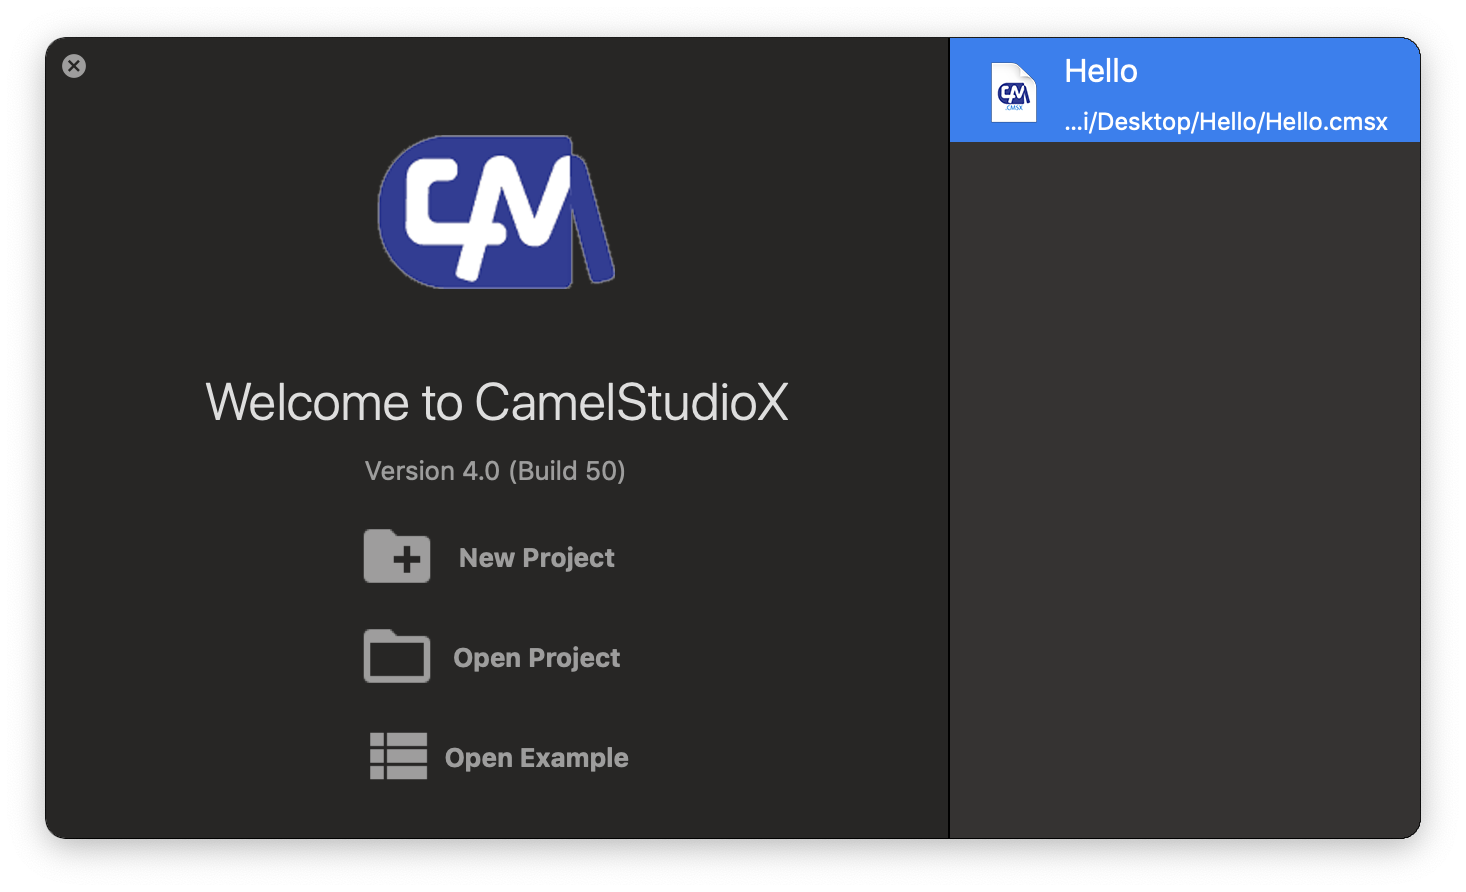
\includegraphics[width=.8\textwidth]{CamelStudioX-Welcome}
		\caption{Welcome Window}
	\end{figure}
		
	The left section shows you the version three buttons to create, open a project or an example project we provide.
	The right section is a project inspector that shows projects you recently create and edit. You can simply double click a project  to open it.
		
	\section{Create a new project}
	
	To create a new project, you can just simply click \textbf{New Project} in the \textbf{Welcome Window}, choose \textbf{New} in the \textbf{Main Menu} or just use key shortcut \textbf{Command + N}.

	\begin{figure}[h]
		\centering
		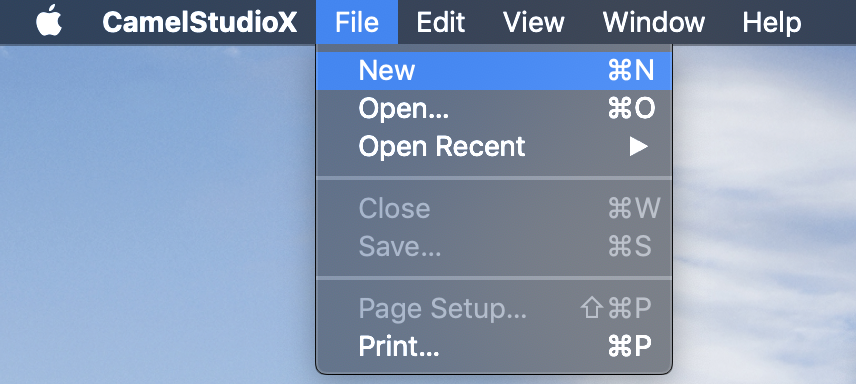
\includegraphics[width=.8\textwidth]{MainMenu}
		\caption{Main Menu of CamelStudioX}
	\end{figure}
		
	\newpage
	Then, type in the project name you like and click \textbf{Save}.
		
	\begin{figure}[!h]
		\centering
		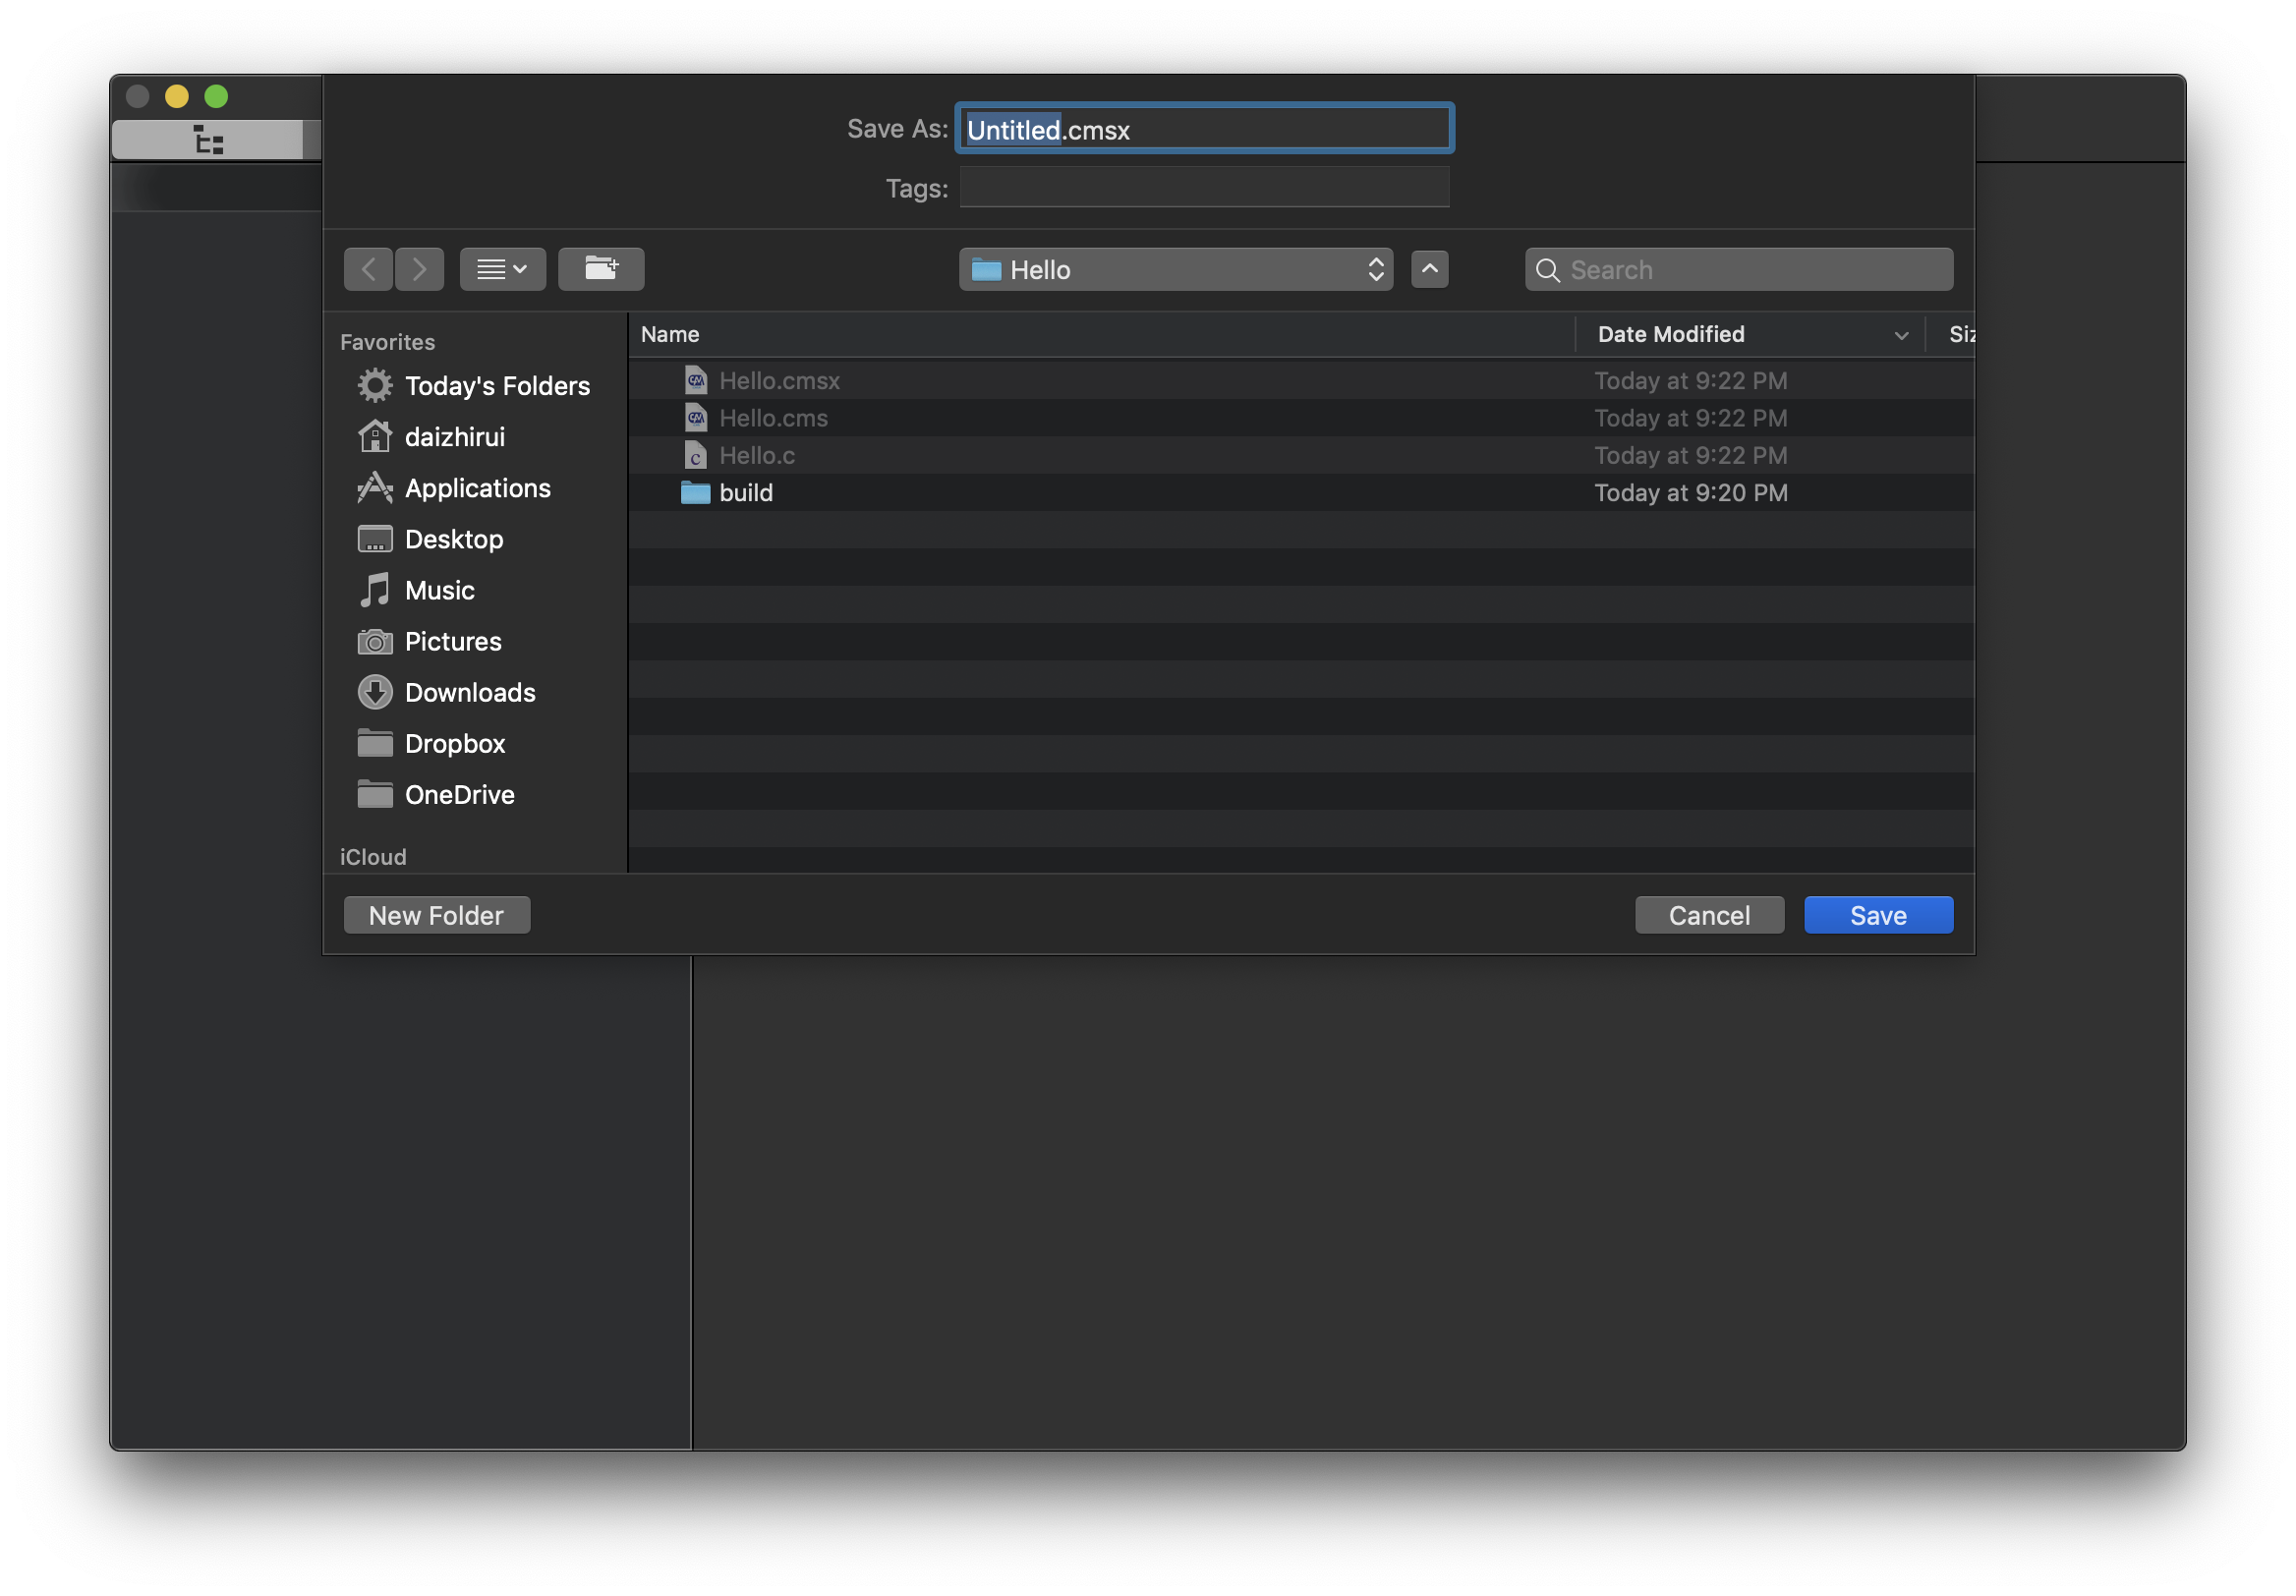
\includegraphics[width=.8\textwidth]{CreateProject}
		\caption{Create a new project}
	\end{figure}
		
	\section{Main Window}
		
	The \textbf{Main Window} is consist of \textbf{Side Panel} and \textbf{Editor Area}.
		
		\subsection{Side Panel}
		In the \textbf{Side Panel}, you can switch three tools \textbf{File Manager, Project Setting and Serial Monitor} by simply clicking different button on the top of the \textbf{Side Panel}.
		
			\begin{figure}[h]
				\centering
				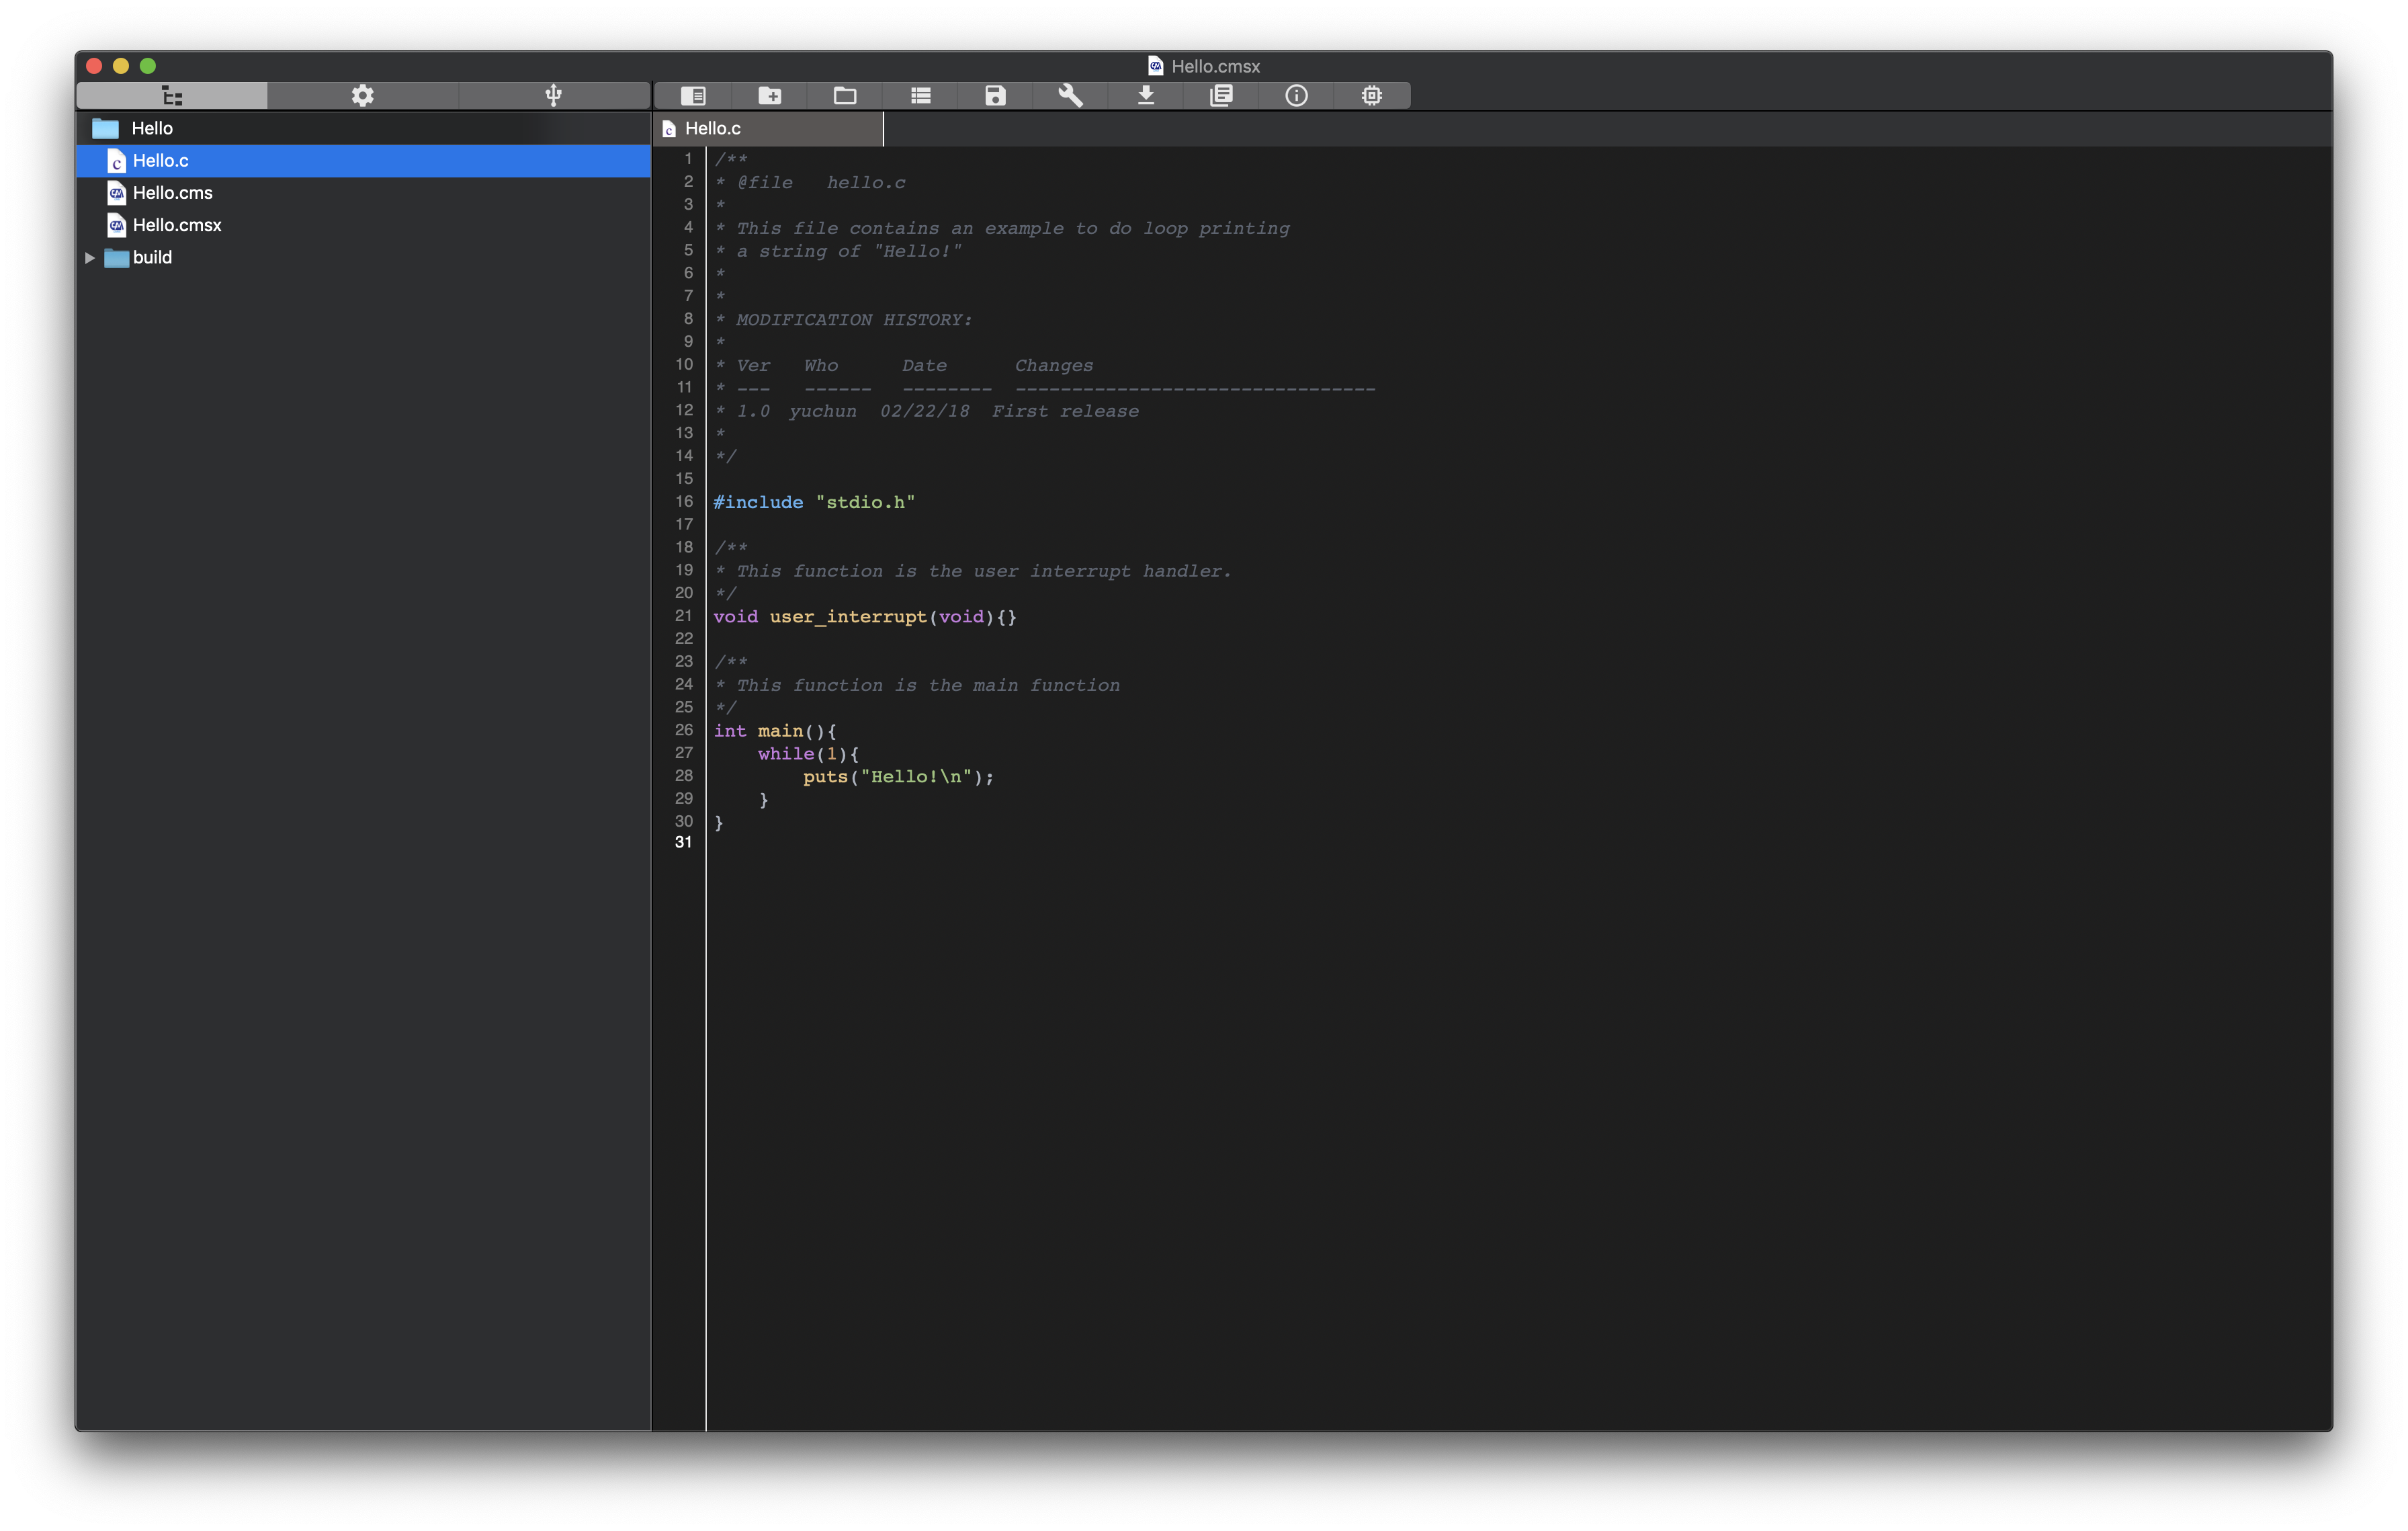
\includegraphics[width=.7\textwidth]{MainWindow1}
				\caption{Main Window with File Manager}
			\end{figure}
		
		\newpage
			\begin{figure}[h]
				\centering
				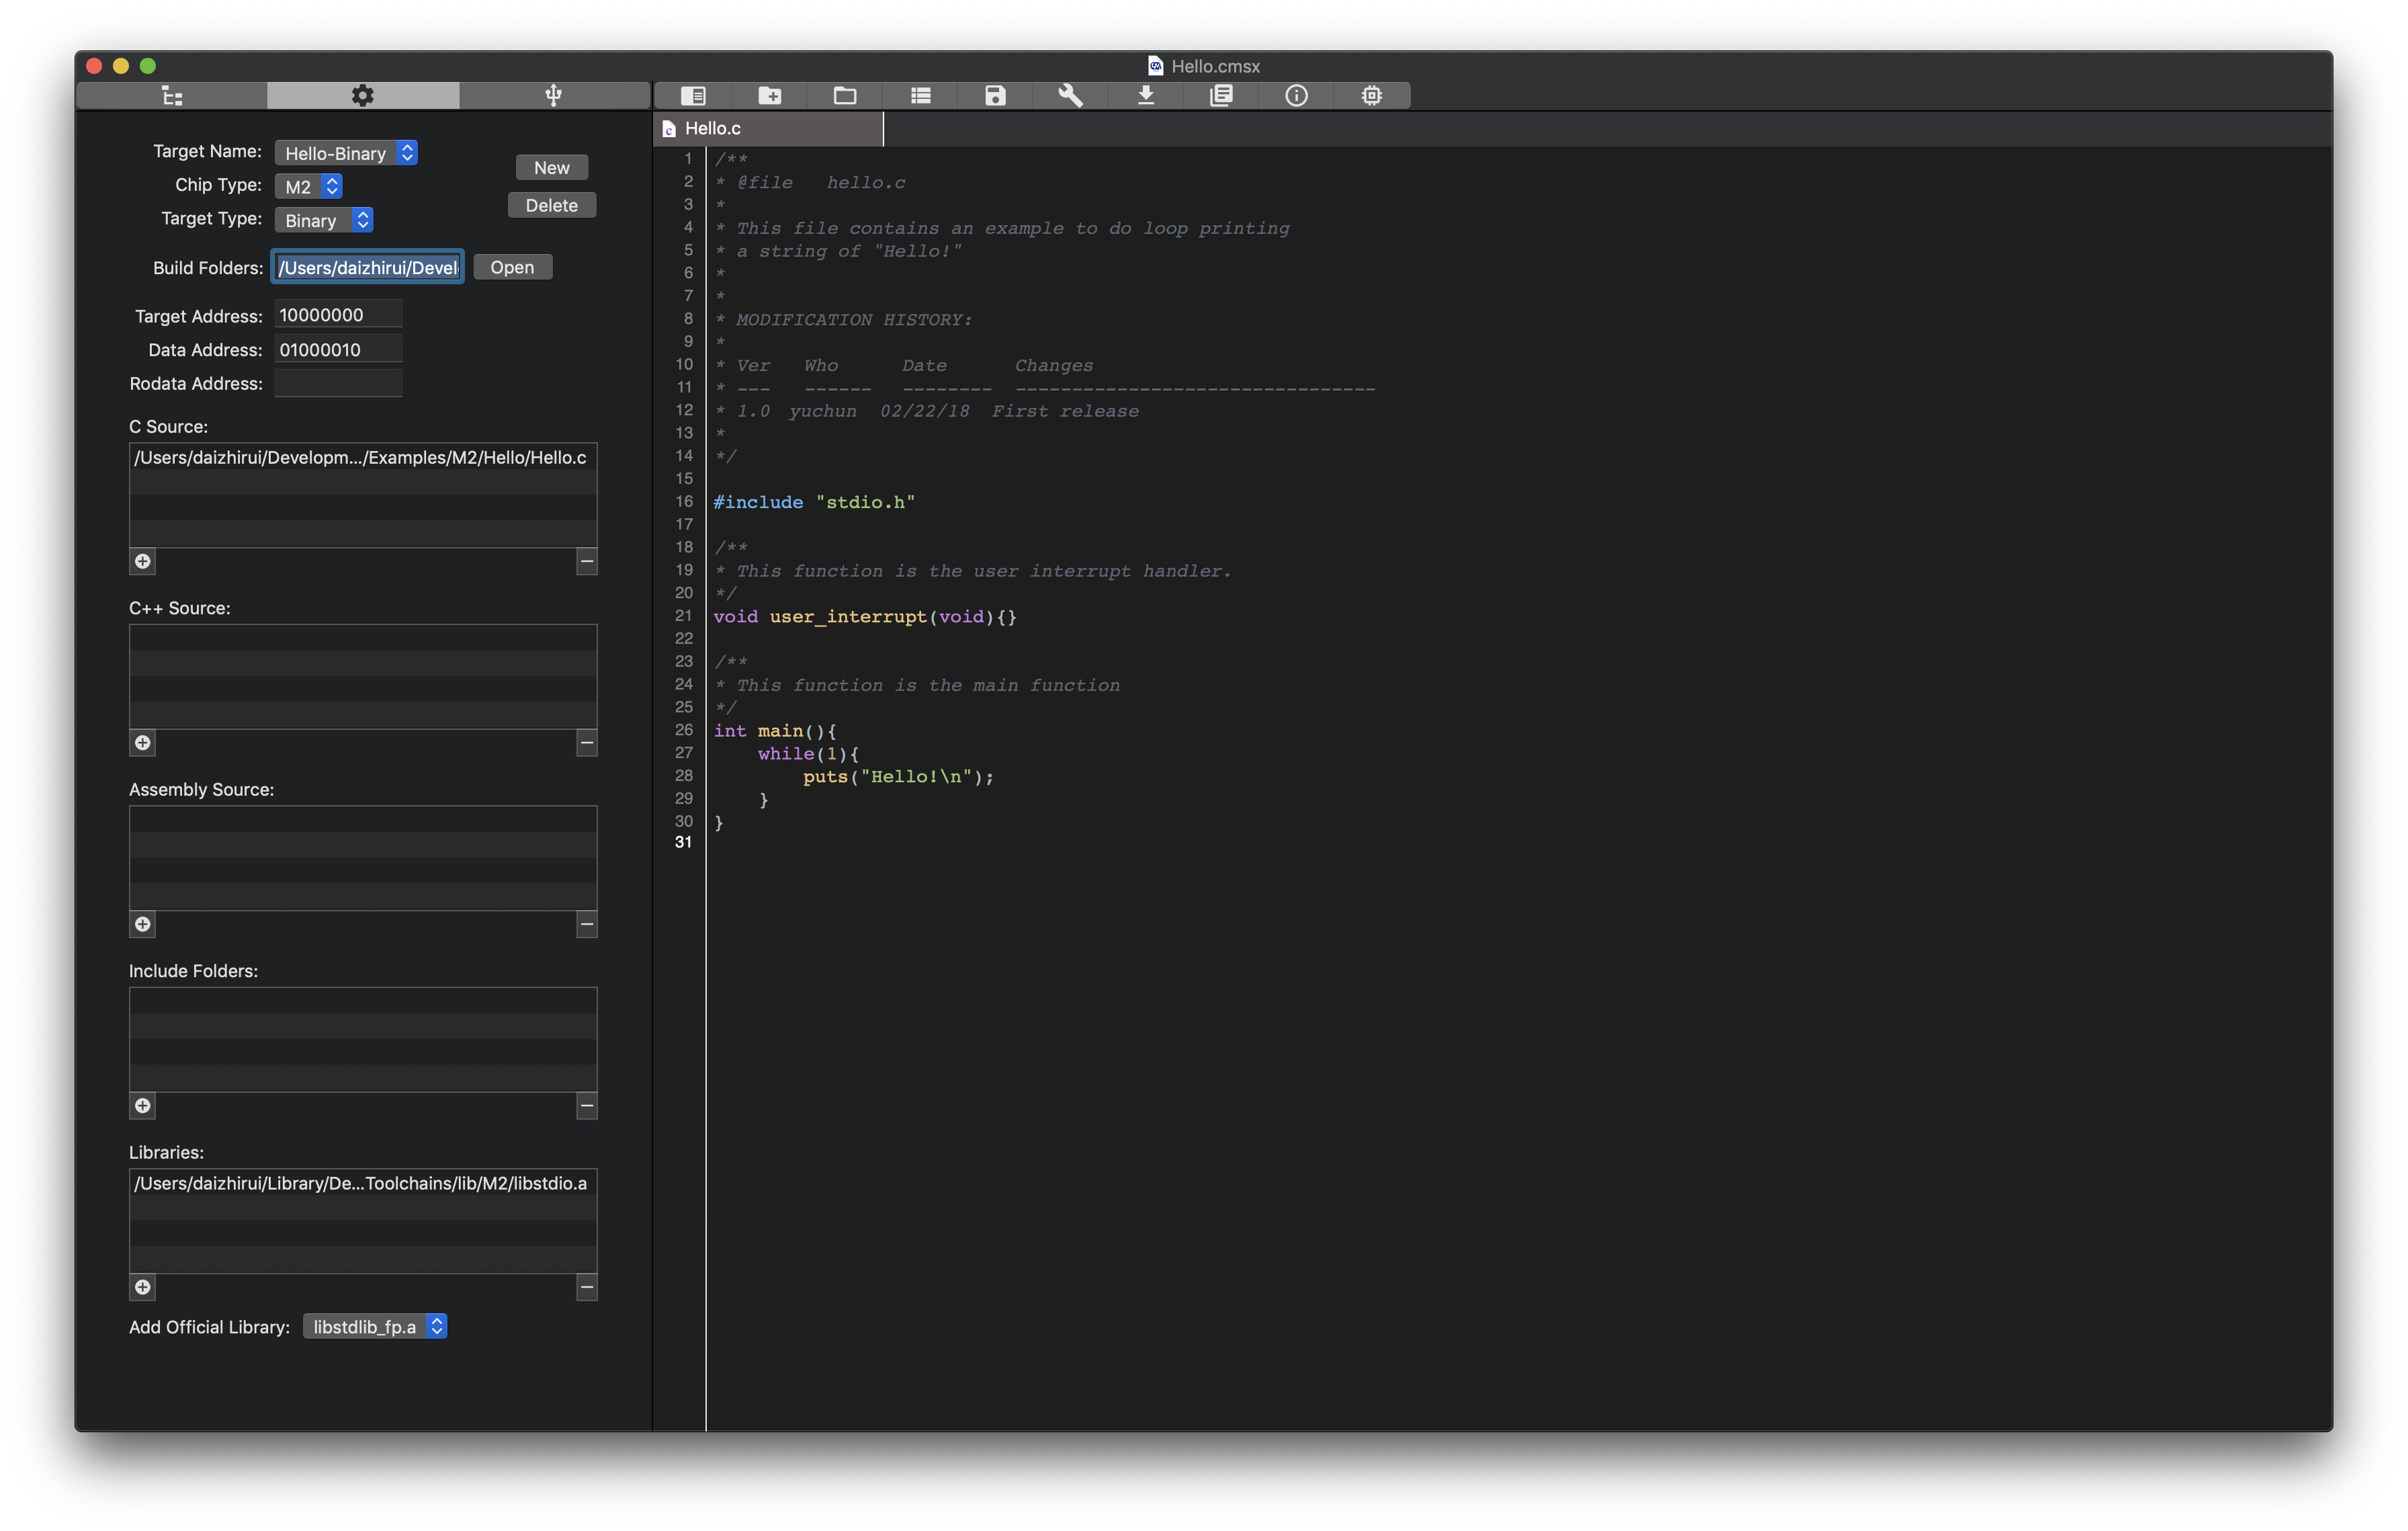
\includegraphics[width=.7\textwidth]{MainWindow2}
				\caption{Main Window with Project Setting}
			\end{figure}
		
		\subsubsection{Project Setting}
			\begin{enumerate}
				\item Choose a target you want to build or create a new target.
					\begin{figure}[!h]
						\centering
						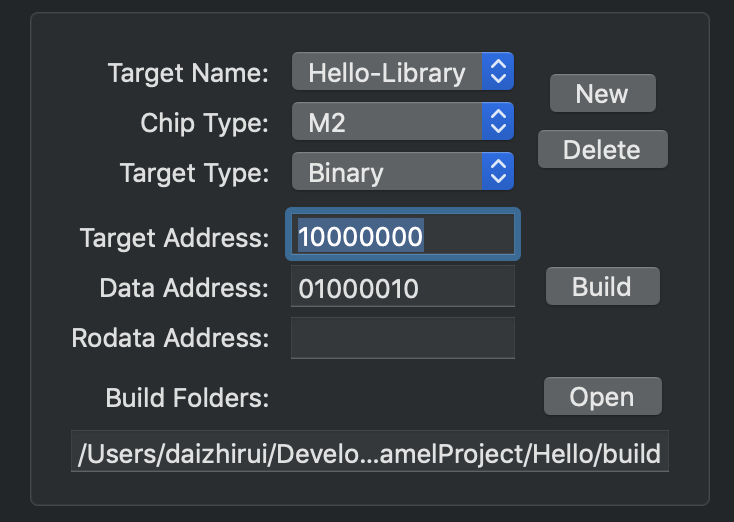
\includegraphics[width=.6\textwidth]{ProjectSetting-1}
						\caption{Target Box of Project Setting}
					\end{figure}
					\newline
					For every target, you should specify at least the \textbf{Target Address, Data Address and Build Folders} to make the target buildable.
					
				\item Add C, C++, assembly, include folders, libraries to different tables respectively.
					\newline
					Under the target box showed above, there are 6 tables. The first 5 tables are for adding \textbf{C, C++, assembly, include folders and libraries} respectively.
					\newpage
					\begin{figure}[!h]
						\centering
						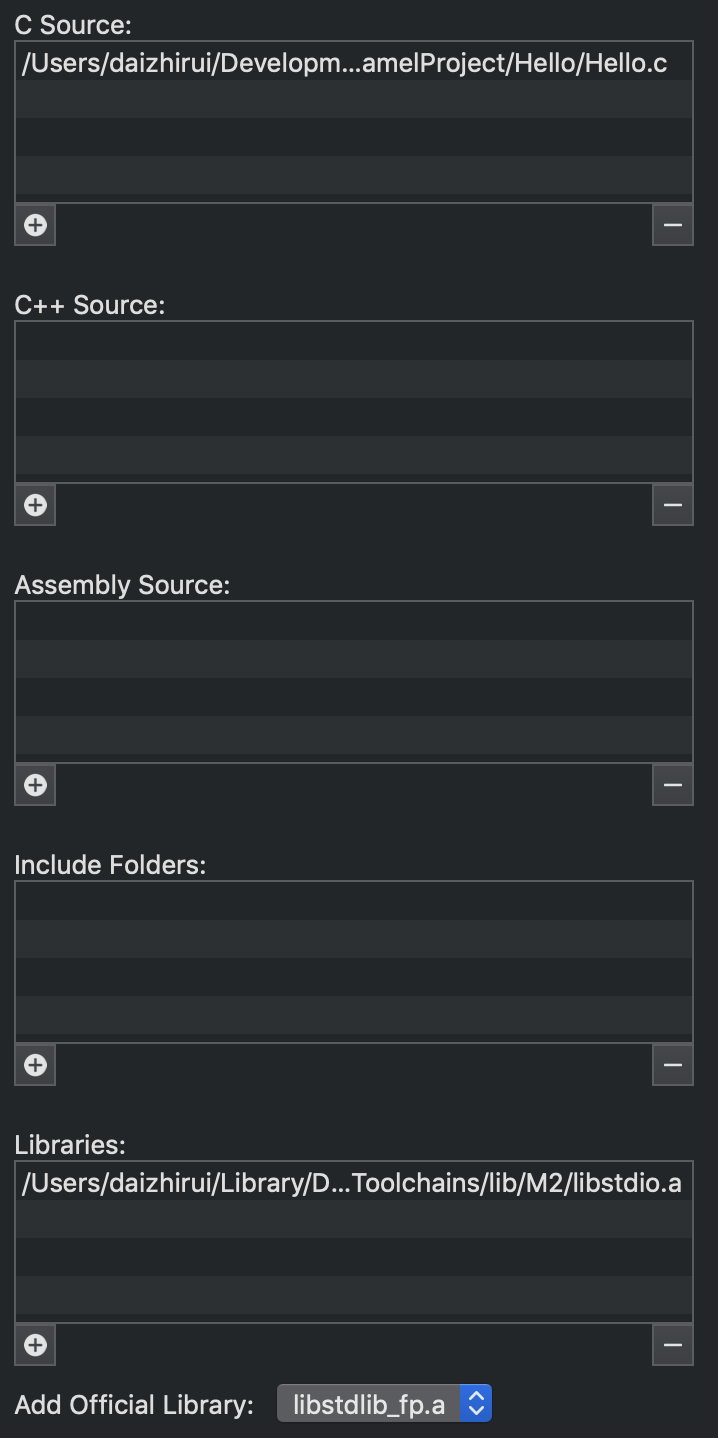
\includegraphics[width=.4\textwidth]{ProjectSetting-2}
						\caption{File Tables of Project Setting}
					\end{figure}
					
					To add official libraries, click the button under the library table. This button will update its content when \textbf{Chip Type} is changed.
				\item Now you can click \textbf{Build Target} button in the \textbf{Editor Area} if you want to build the target you select and setup just now.
					\begin{figure}[h]
						\centering
						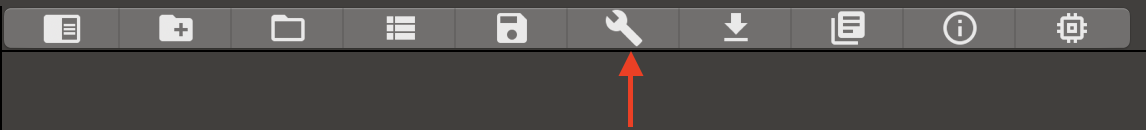
\includegraphics[width=.5\textwidth]{ToolBar-Build}
						\caption{Click to Build the Selected Target}
					\end{figure}
				
				\item You may want to build more than one target together. Switching between different targets and clicking the build button is very inconvenient. Well, the 6th table will satisfy your requirement.
					\begin{figure}[!h]
						\centering
						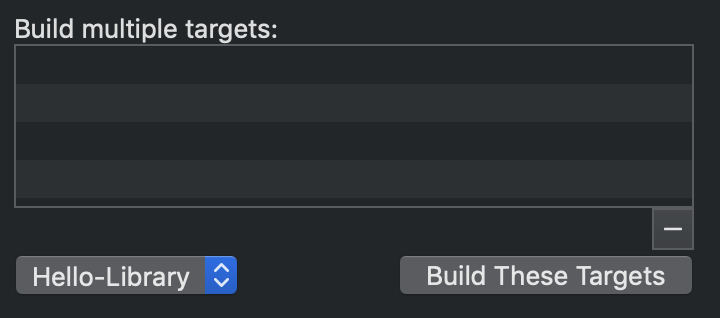
\includegraphics[width=.4\textwidth]{ProjectSetting-3}
						\caption{Build Multiple Targets}
					\end{figure}
					\newline
					You can choose a target and add it from the button at the left-bottom corner. And then click the \textbf{Build These Targets} button.
					
			\end{enumerate}
			
		\newpage
		\subsubsection{Serial Monitor}
		
			\begin{figure}[h]
				\centering
				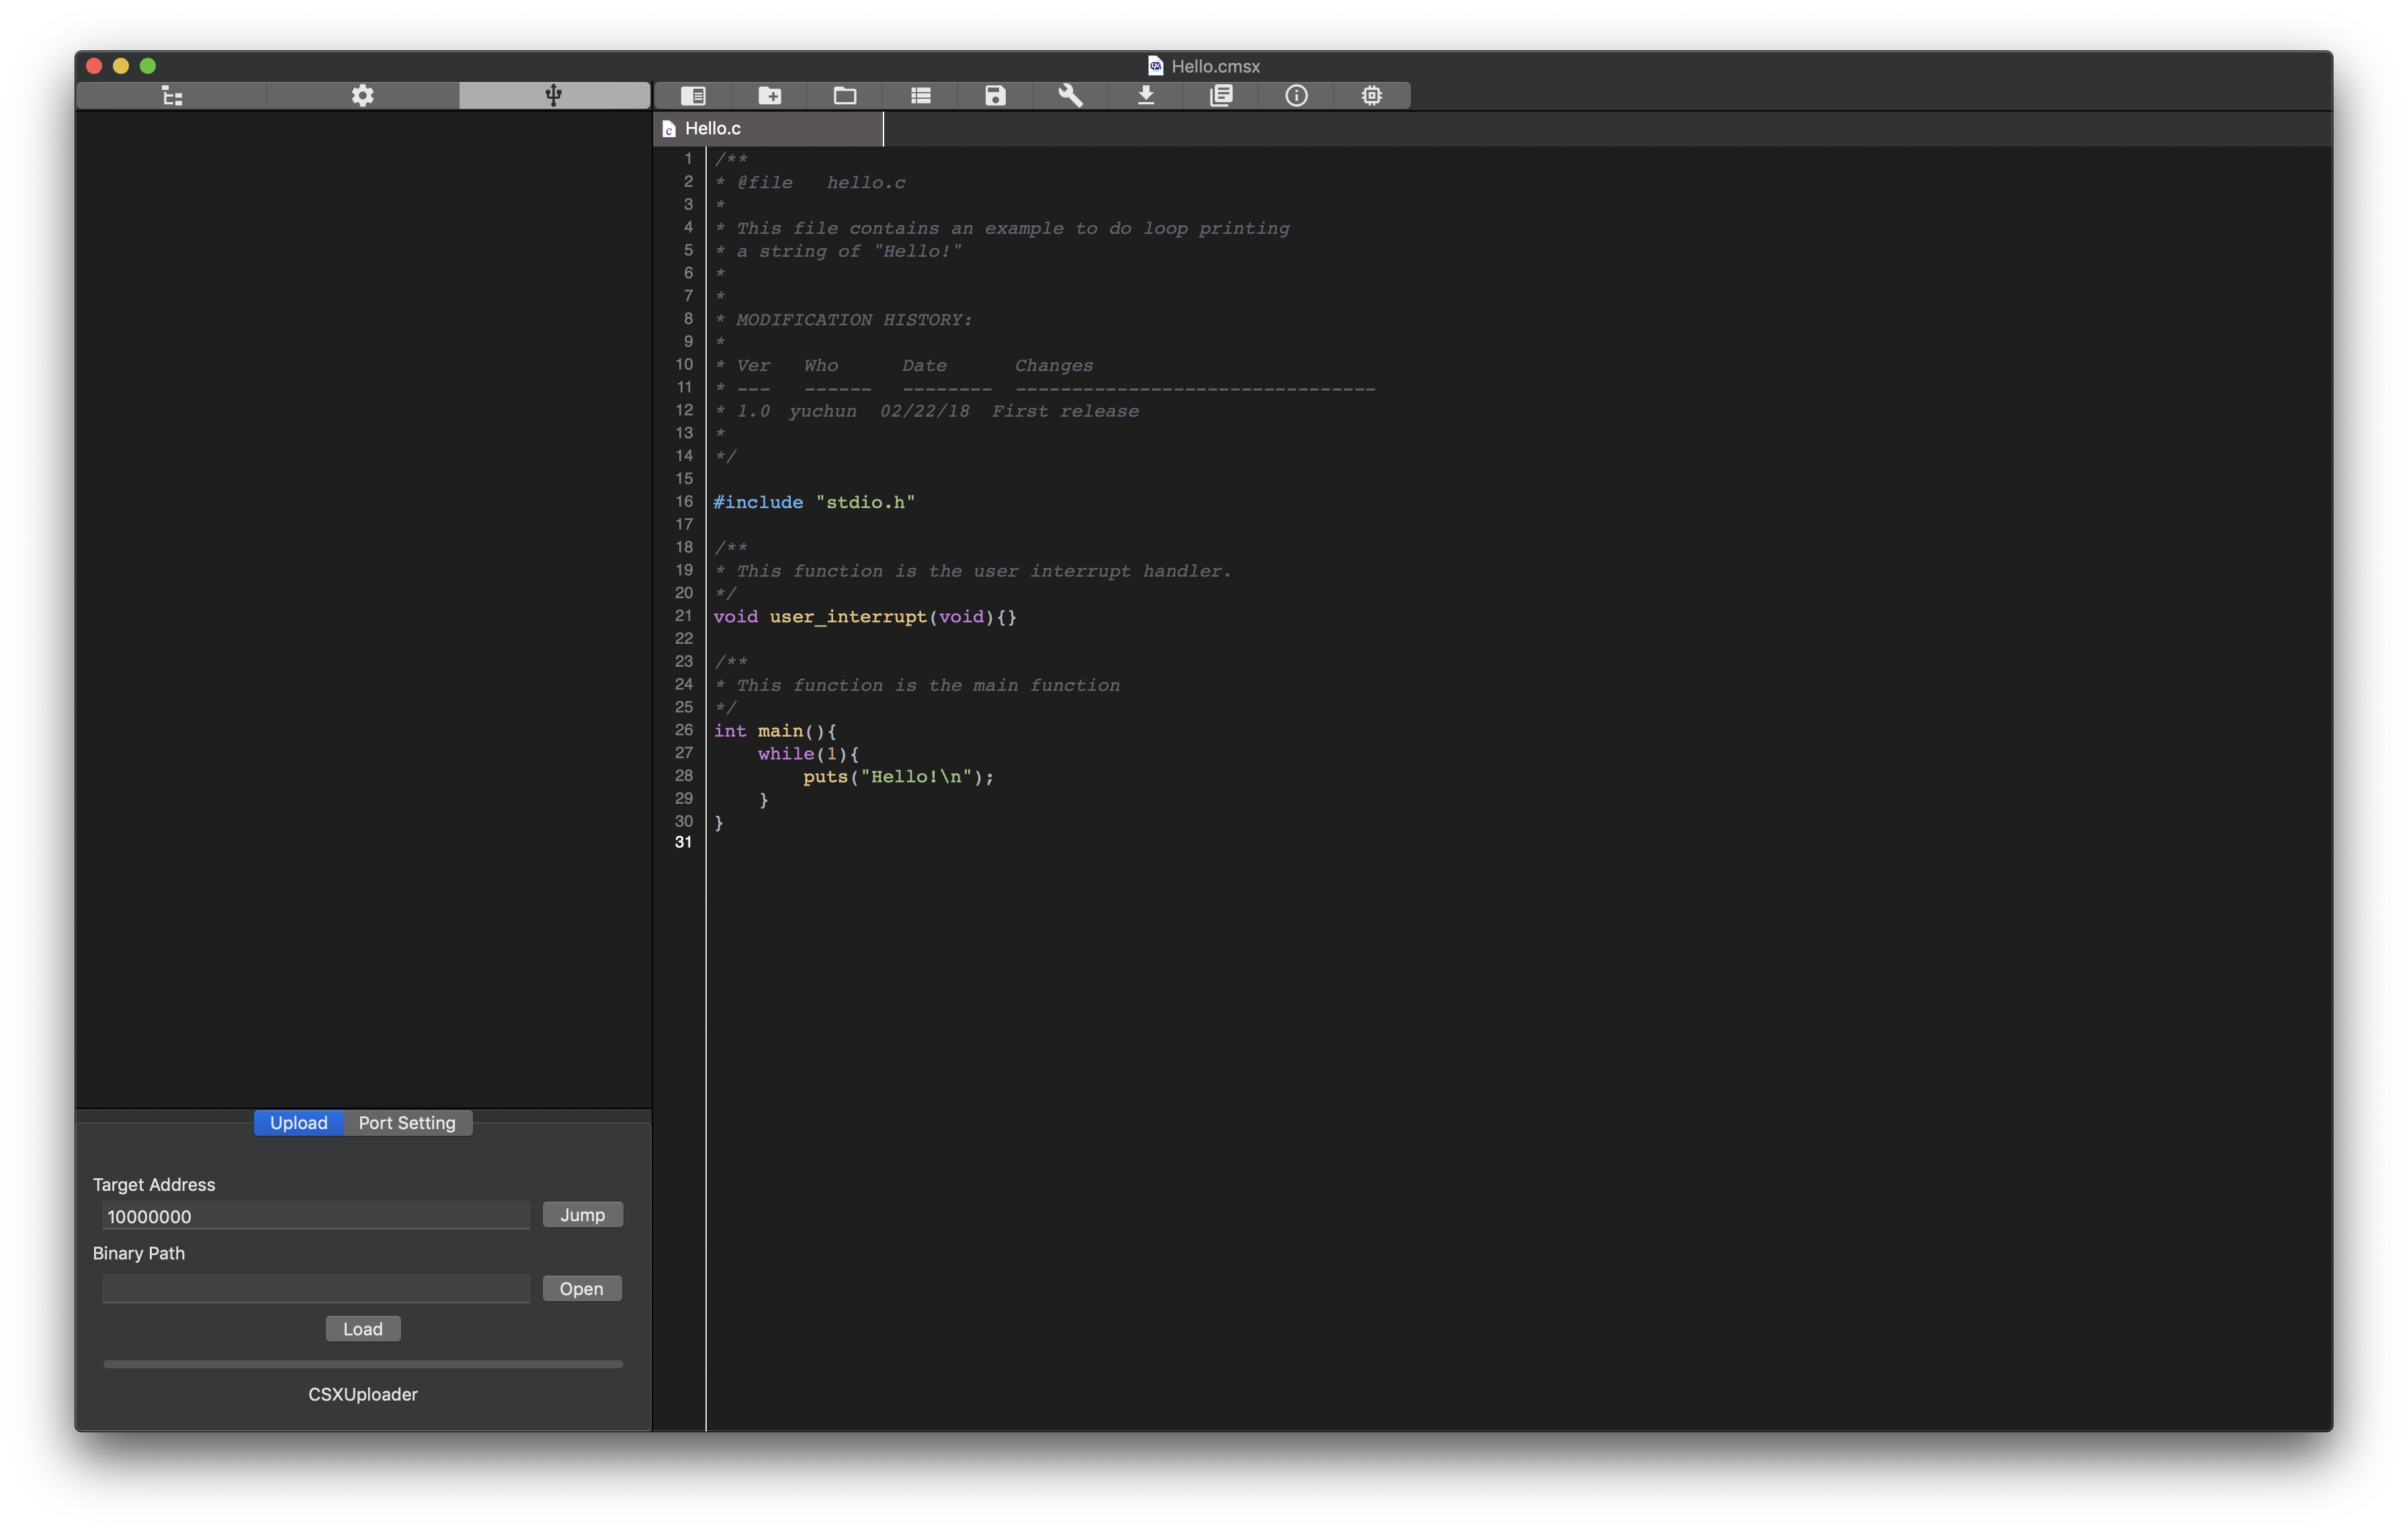
\includegraphics[width=.65\textwidth]{MainWindow3}
				\caption{Main Window with Serial Monitor}
			\end{figure}
		
			In \textbf{Serial Monitor}, you can not only receive the output from the chip via serialport, but also upload a specific binary to the chip with a specific target address.
			
			\begin{figure}[h]
				\centering
				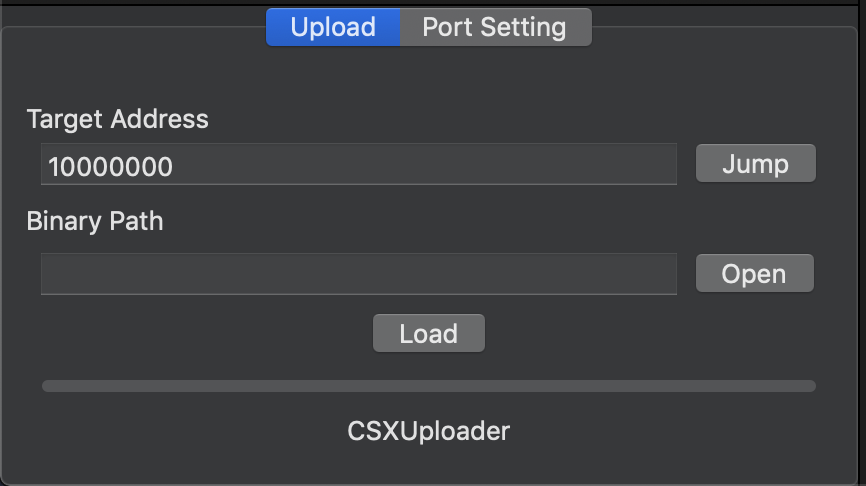
\includegraphics[width=.49\textwidth]{SerialMonitor1} \hfill
				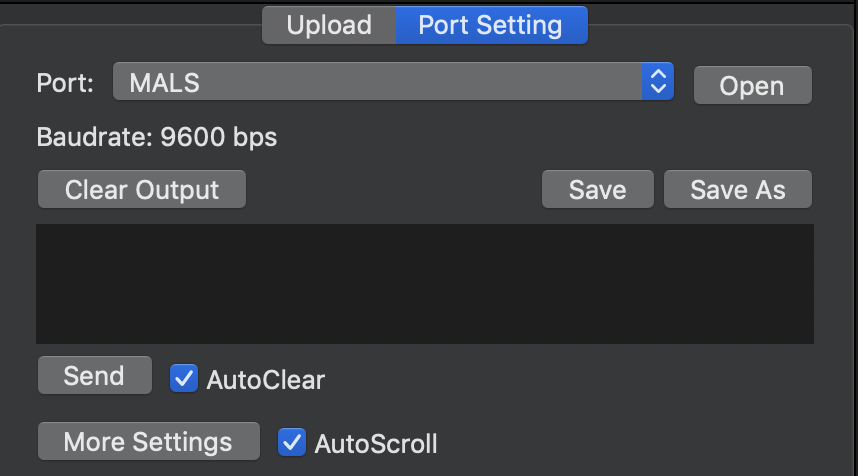
\includegraphics[width=.49\textwidth]{SerialMonitor2} \hfill
				\caption{Panels for Uploading a Binary and Serial Port Setting}
			\end{figure}
			
			If you cannot find your chip in the port list, you may have to install a suitable serial port driver. Click the \textbf{Install Serial Driver} button in the \textbf{Editor Area} to open the serial driver installation sheet and choose a driver installer you need.
			
			\begin{figure}[h]
				\centering
				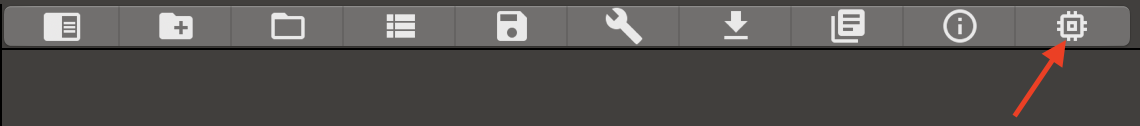
\includegraphics[width=.6\textwidth]{ToolBar-SerialDriver}
				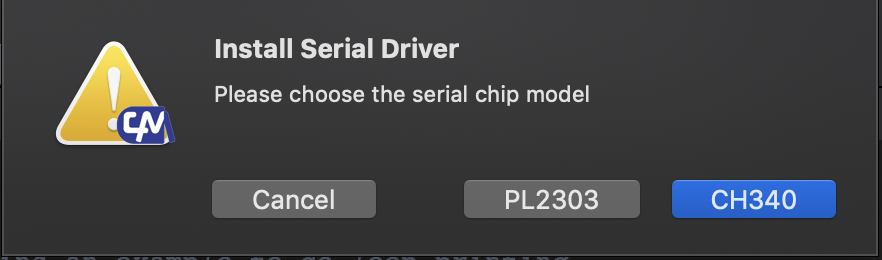
\includegraphics[width=.6\textwidth]{SerialDriver}
				\caption{Install Serial Driver}
			\end{figure}
		
		\newpage
		\subsection{Editor Area}
		
			The integrated editor supports multiple tabs, syntax highlighting and auto completion suggestion.
			
			To change the syntax highlighting theme, open \textbf{Preference} (key shortcut: Command + ,) and choose a code theme you like.
			
			\begin{figure}[h]
				\centering
				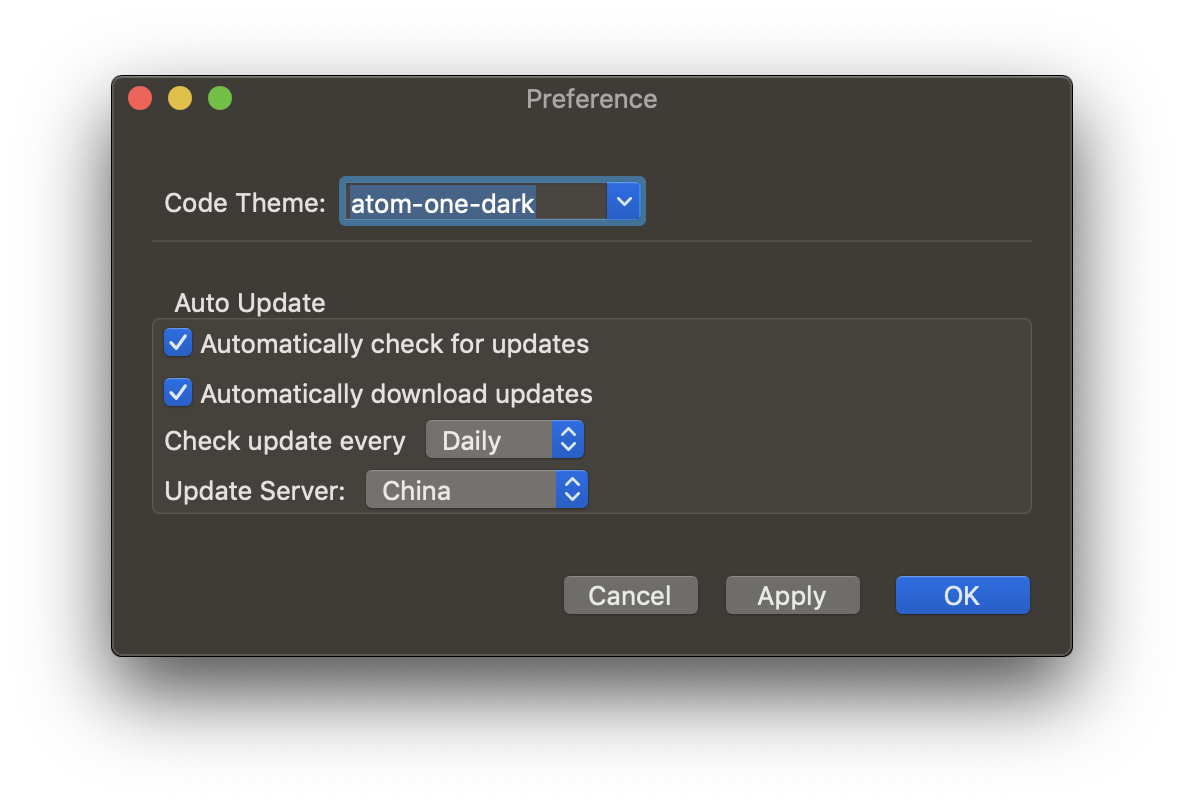
\includegraphics[width=\textwidth]{Preference}
				\caption{Preference of CamelStudioX}
			\end{figure}
			
			There is a tool bar at the top. The function of each button is showed below.
			
			\begin{figure}[h]
				\centering
				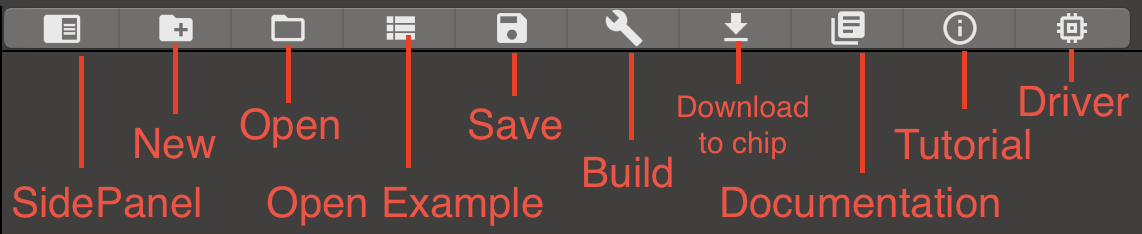
\includegraphics[width=\textwidth]{ToolBar}
				\caption{Toolbar in Editor Area}
			\end{figure}
			
	\newpage
	\section{Documentation}
	
		If you have any question about the official library, you can check the documentation at first.
		
		\begin{figure}[h]
			\centering
			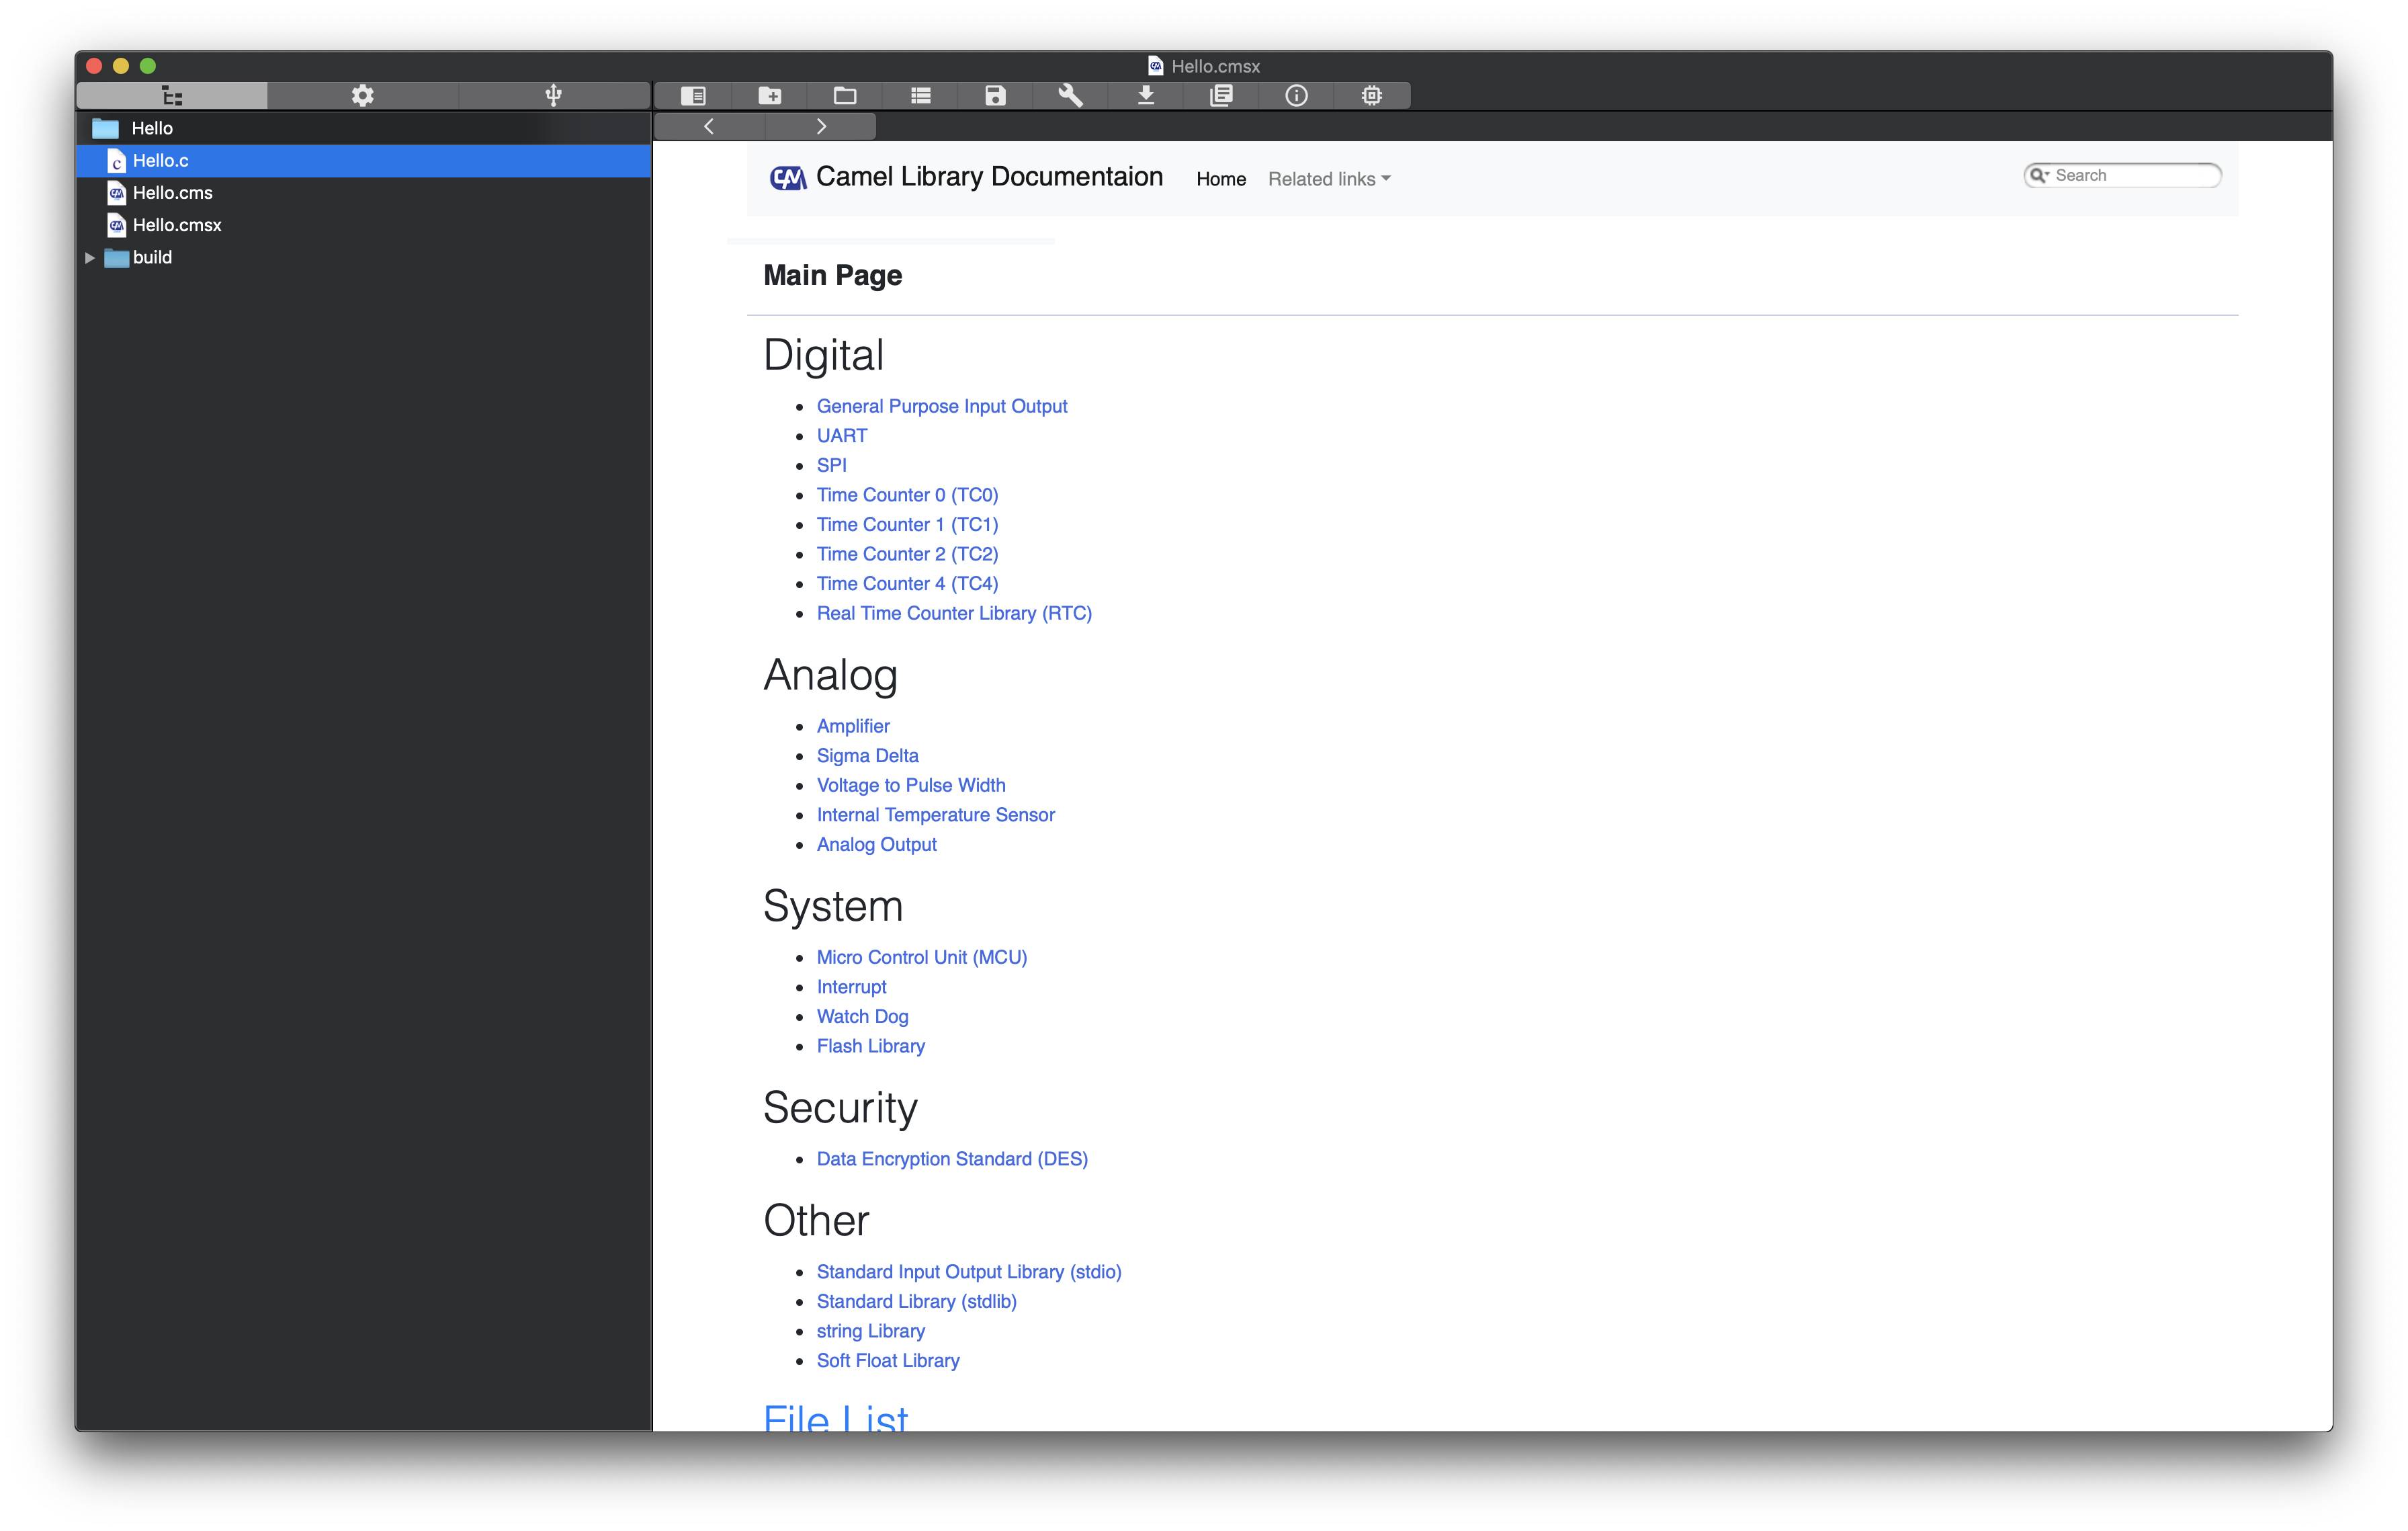
\includegraphics[width=\textwidth]{Documentation}
			\caption{CamelStudioX Documentation}
		\end{figure}
		
	\newpage
	\section{Dark Mode for macOS ${\geq10.14}$}
	
		For users who use macOS Mojave or newer version, they can switch between \textbf{Light Mode} and \textbf{Bold Mode} in the \textbf{System Preference - General} panel.
		\textbf{CamelStudioX} is adapted to macOS Mojave and it supports dark mode according to the system setting. This is a system feature. So CamelStudioX cannot provide a dark mode in system older than 10.14 yet.
		
		\begin{figure}[!h]
			\centering
			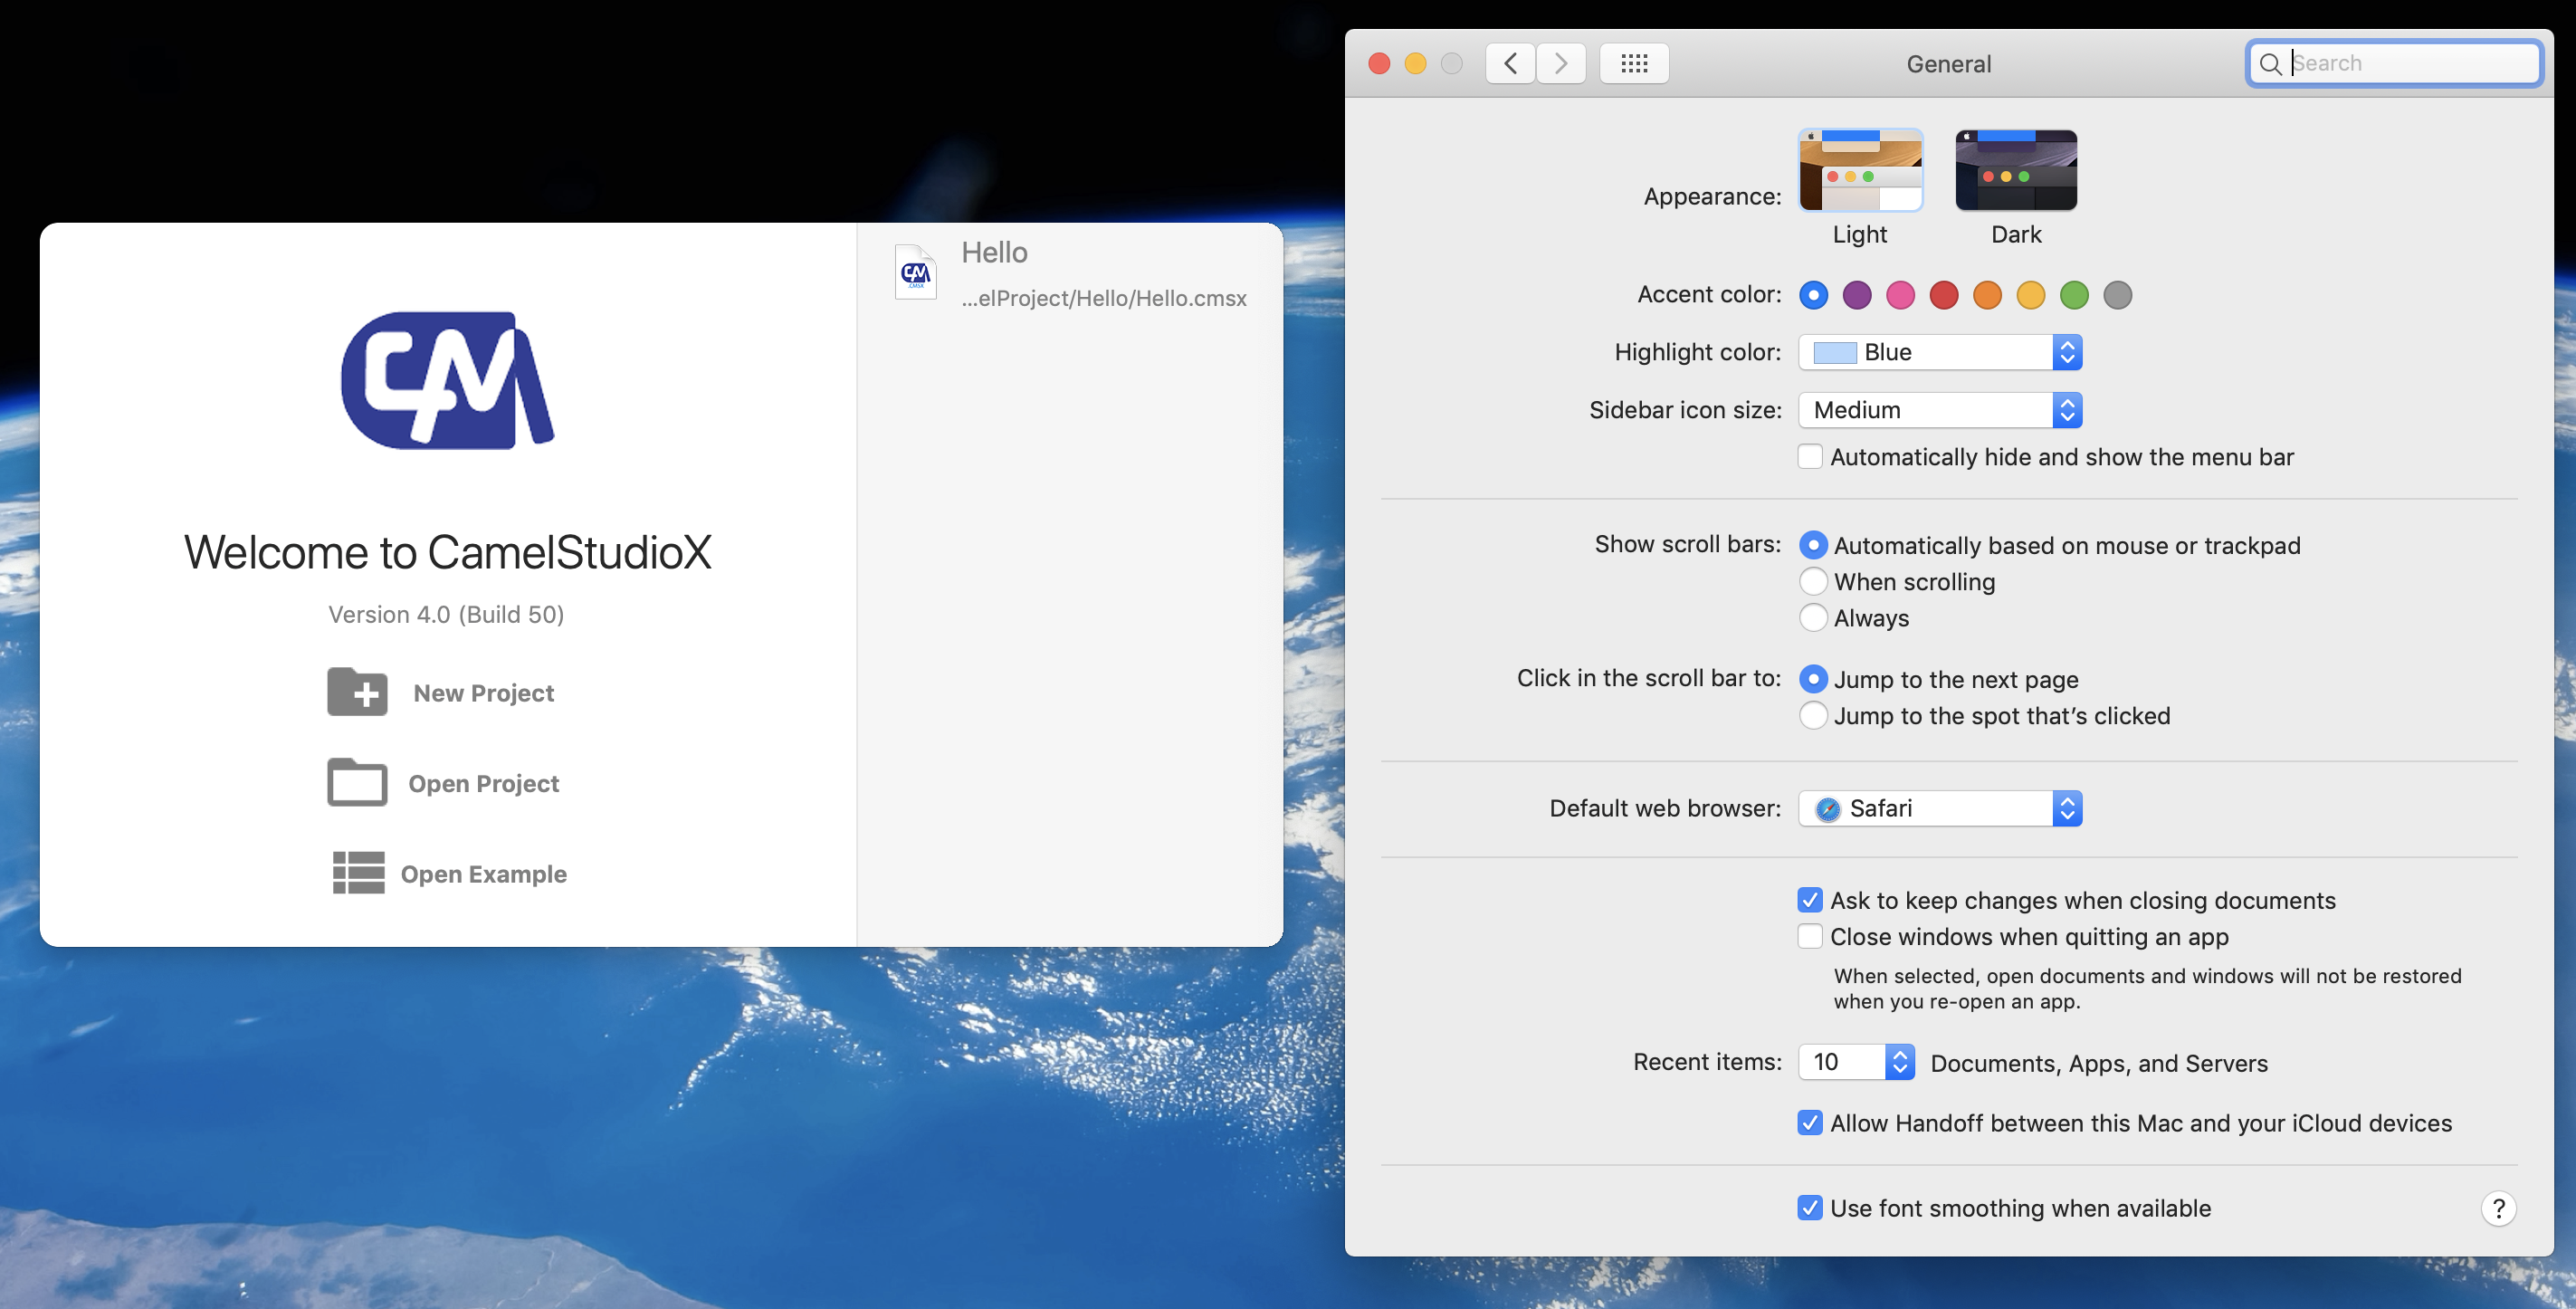
\includegraphics[width=\textwidth]{LightMode}
			\caption{Light Mode}
			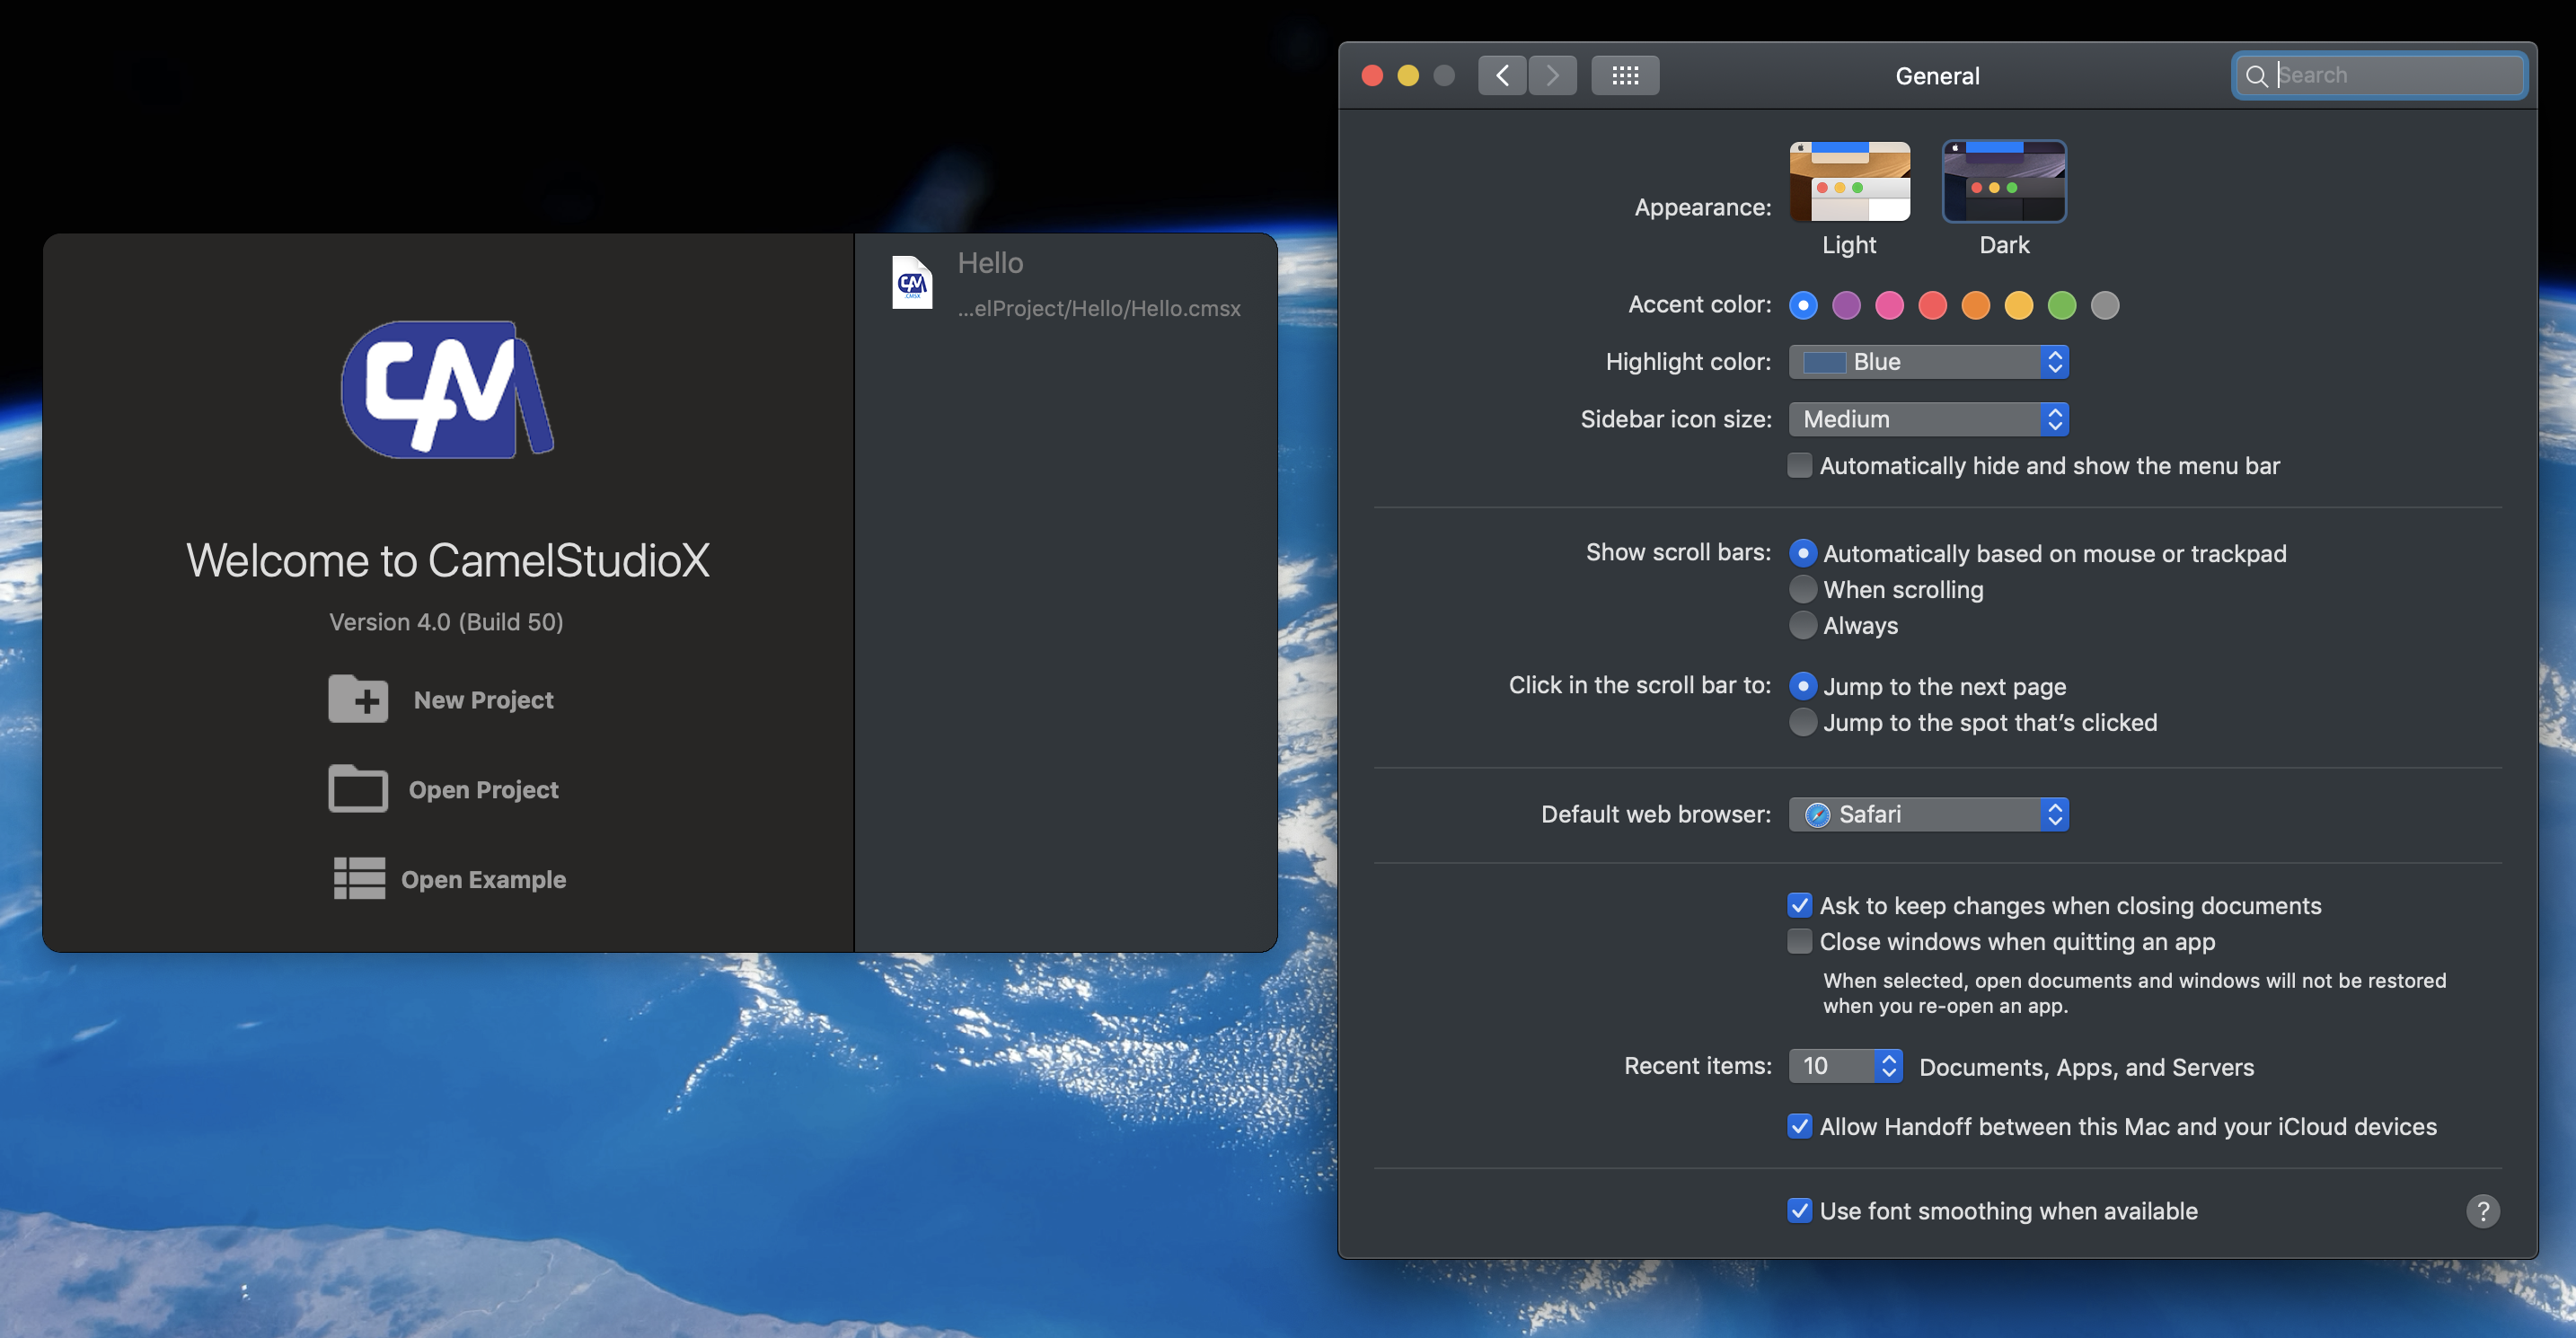
\includegraphics[width=\textwidth]{DarkMode}
			\caption{Dark Mode}
		\end{figure}
\end{document}